\documentclass[12pt]{report}
\usepackage{lipsum}
\usepackage{mathtools}
\usepackage{array}
\usepackage{colortbl}
\usepackage{chemfig}
\usepackage{csvsimple}
\RequirePackage[left=3cm,top=1.5cm,right=3cm,bottom=2.5cm,nohead]{geometry}
\usepackage{sectsty}

\sectionfont{\fontsize{17}{15}\selectfont}

\begin{document}

\begin{titlepage}
	\begin{center}
		\vspace*{1cm}
		
		{\Huge \textbf{Social distancing detection with computer vision techniques}}
		\vspace{2mm} \\
{\LARGE 
		\vspace{2mm}
		\textbf{by Lee Hoang}}
		\vspace{2mm}
	
		
		\vspace{1.5cm}
		
		\vfill
		{\Large \textbf{Project supervisor: Dr Cristina Gacek}}
		
		\vspace{0.8cm}
		
{\Large 		\textbf{BSc Computer Science\\
		City, University of London\\
		Academic Year: 2020-21\\}}
		
	\end{center}
\end{titlepage}

\tableofcontents


\pagebreak

\chapter*{Abstract}

The project aims to detect social distancing between pedestrians using computer vision techniques. Each video input generates different coloured bounding boxes for each person depending on their social distancing status. The system allows small offices to monitor their worker's movement and grants face-to-face communication at a safe distance.

\vspace{2mm}
The report discusses three solutions which includes calibrated cameras to calculating social distancing within an image or video and an in depth analysis on how different camera qualities affect the output of the system. An additional feature is added to detect groups of people who enter the frame of the camera to allow people to walk in groups. 


\chapter{Introduction}

\section{Problem solved}

Corona virus has become an issue for many countries, resulting in lockdown of many companies and public areas, restricting students and workers from having face-to-face communication with their peers and having to work at home. As a result, it influences the flow of work negatively (Lewis and Kuhfeld, 2021). Social distancing has been used to combat the outbreak of the corona virus to reduce the spread. 

\vspace{2mm}

The purpose of this project is to detect social distancing in a public area from a image or video source, with and without the use of calibrated cameras. The software allows for better surveillance in public areas and workplaces, granting people to have safe contact within an area while having a more productive workflow.

\vspace{2mm}

Three different methods to calculating social distancing are achieved as well as an algorithm developed to detect groups of people who are coming into the frame of the camera. One of the methods discussed is also used in an existing system (Y. C. Hou, 2020) which is discussed in the background research chapter. To build from the existing system's method, the author uses camera calibration to remove distortion within each video frame to produce higher accuracy when calculating social distancing.

\section{Project objectives}

The sub objectives that are presented in the report are different from the sub objectives seen in the PDD. For example, the PDD mentions using two different object detection models to compare speed and accuracy. In the end, the report only used the 'yolov3' model for object detection. The primary objective still remains the same.

\subsection{Primary objectives}

Detect and calculating social distancing between pedestrians. Mark people within the dataset who are not 'social distancing' with a red bounding box, otherwise mark the person with a green border. The final output must have a top down view/plot of the pedestrians which is in sync of the video used.

\subsection{Sub objectives}

\noindent
1 - Detect a human being within a frame of a video using OpenCV. Later detect the human being moving in the video. Goal is to display a bounding box around the person and add a label to identify that they are human.

\vspace{2mm}

\noindent
2 - Produce an analysis on how the 'yolov3' architecture performs under different camera qualities by adding artificial noise and resizing the resolution of the image/video. 

\vspace{2mm}

\noindent
3 - Calculate the distance between two people by pixels. Also calculating the distance with the use of calibrated cameras for greater accuracy.

\vspace{2mm}

\noindent
4 - Create a top-down view/plot of the people in the video, identifying their location and proximity to others nearby. The program will display a top-down transformation that maps the people we have detected. The display will be in sync with the video.

\vspace{2mm}

\noindent
5 - Identify groups of people who are close in the dataset as “safe distancing”. The test for this is to allow groups of people to be “safe” when close as they are recognized as friends or family.


\section{Project Beneficiaries}

This project helps office workers and small businesses to have safe face-to-face contact as the system will monitor their distance from each other. While the project does not include a real time camera, the program can be changed to do so and still maintain the core functionality of calculating social distancing. The system may be applicable to a small class within a school, this allows students to interact with their teachers and school equipment.

\section{Work performed}

The primary and sub objectives discussed in section 1.2 has been completed. The system is able to calculate social distancing within an image or video and mark pedestrians with the corresponding coloured bounding boxes. The fifth sub objective is seen as an optional task as a complete solution is very complex, therefore the task was completed to a satisfactory level.


\section{Assumptions}

The object detection used (YOLO) has limitations in what it can detect depending on the position of the object. For example, the model has trouble detecting a person hiding behind another person. This leads to the report giving leniency to the model and disregards most mistakes that 'yolov3' outputs. This is further discussed in section 5.1.

\chapter{Output Summary}

\section{Social distancing detector application}

\begin{tabular}{|p{2.2cm}|p{11cm}|}
	\hline
	Description & The source code for the social distancing detector\\
	\hline
	Output Type: & The project source code contains 9 python files that comprises of approximately 700 lines of code. Approximately 20 lines of code was adapted from an external source which is loading the 'yolov3' model using OpenCV functions.  \\
	\hline
	Usage: & User is able to input an image or video and the system will calculate social distancing between the people within the input and output a plot that represents the top down view of the input. \\
	\hline
	Recipient: & Author and beneficiaries \\
	\hline
	Appendix Link: & GitHub link: 
	
	https://github.com/lhoang247/Individual-Project \\
	\hline
\end{tabular}

\section{Screenshots of the system's development}

\begin{tabular}{|p{2.2cm}|p{11cm}|}
	\hline
	Description & Screenshots of the WILDTRACK dataset with additional drawings using OpenCV added by the system\\
	\hline
	Output Type: & The system produces images/frames that are converted to screenshots by the author. The file type is either JPG or PNG  \\
	\hline
	Usage: & The images are the outputs of the system from early stages of the development to provide the reader with visual examples of what the system outputs. \\
	\hline
	Recipient: & Author and reader \\
	\hline
	Appendix Link: & The results chapter, Appendix 4, 5, 6, 7. GitHub link: 
	
	https://github.com/lhoang247/Individual-Project/tree/main/report/images \\
	\hline
\end{tabular}

\pagebreak

\section{Video outputs from the system}

\begin{tabular}{|p{2.2cm}|p{11cm}|}
	\hline
	Description & Videos of the WILDTRACK dataset with additional drawings using OpenCV added by the system\\
	\hline
	Output Type: & The system outputs a video and is saved using OpenCV functions \\
	\hline
	Usage: & The videos provide visual examples of the system outputs. \\
	\hline
	Recipient: & Author and reader \\
	\hline
	Appendix Link: & The results chapter, Appendix 4, 5, 6, 7. GitHub link: 
	
	https://github.com/lhoang247/Individual-Project/tree/main/report/images \\
	\hline
\end{tabular}

\section{Demonstration video/presentation of system and code}

\begin{tabular}{|p{2.2cm}|p{11cm}|}
	\hline
	Description & Video showcasing the functionality and code of the system.\\
	\hline
	Output Type: & The video is recording using OBS and is formatting to a mp4 file.  \\
	\hline
	Usage: & The video presents and explains part of the code to the reader for better understanding of the system. \\
	\hline
	Recipient: & Author and reader \\
	\hline
	Appendix Link: & Moodle submission \\
	\hline
\end{tabular}

\section{UML Diagrams}

\begin{tabular}{|p{2.2cm}|p{11cm}|}
	\hline
	Description & UML diagrams showcasing the functionality of the overall system.\\
	\hline
	Output Type: & Diagrams are .PNG files that are imported to the report.  \\
	\hline
	Usage: & The diagrams give clarification to the reader about the overall design of the system. It is also a method of planning for the author. \\
	\hline
	Recipient: & Author and reader \\
	\hline
	Appendix Link: & The method chapter, Appendix 2, 3 \\
	\hline
\end{tabular}

\chapter{Background Research}

\section{What is computer vision?}

Computer vision (CV) is a scientific discipline that studies how computer can efficiently perceive, process, and understand information from visual data such as images and videos.

\vspace{2mm}

As humans, we can classify three-dimensional objects with ease, whether the pictures are the same object with different colours or angles, we are good at determining the object we are classifying. 
Computer vision has been developed to detect edges from a pixelated image, face detection, and has been used to develop 3D models from a snapshot yet the technology we have today could be compared to a young child's biological vision. 
Computer vision is used in various real world application such as traffic surveillance or medical imaging (SZELISKI, 2020), where people are now able to utilize magnetic resonance imaging (MRI) to safely analysis the heart wall motion where the end result is a 3d model of the heart pumping (Metaxas, 1997). 

\vspace{2mm}

In recent years, computer vision has been adapting deep learning algorithms to efficiently classify unseen objects within pixel images and videos. 


\section{Deep learning}

Deep learning uses artificial intelligence (AI) to try and simulate the choices that a human brain will make. Problems that have regression or classification outputs can be solved by passing data/inputs through artificial neurons which were previously tweaked for the specific problem by training data. There are many different variants of deep learning algorithms such as Artificial Neural Networks (ANN) or Long Short-Term Memory (LSTM) Networks (Hochreiter, 1997) which build onto each other.

\subsection{Neural networks (NN)}

Neural networks is a network formed of interconnected perceptrons which each carry weights and biases. The weights (w) and biases (b) are each represented by a float value which are used to multiply and add to the input respectively. The output from the weight and bias is then put into an activation function (e.g. ReLU or sigmoid) which determines if the neuron should be activated. These activations chain together to output a value of what the neural network thinks the solution is. 

\vspace{5 mm}

\begin{centering}
	
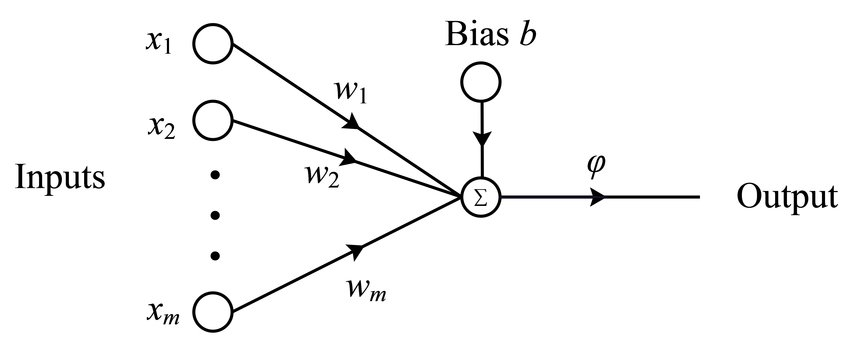
\includegraphics[width=100mm]{./images/weights and biases.png}

{Figure 1: A single perceptron with inputs, weights, and biases}

\end{centering}

\vspace{5 mm}

The values of weights and biases are updated when training data is pass through the network using back propagation, adjusting their values depending on the actual and network's solution to the problem. A network can have multiple layers of several perceptrons in order to solve more complex problems, but has the down side of overfitting the accuracy of the output.


\subsection{Convolutional neural networks (CNN)}

CNNs builds upon the NN, specialising in working with grid-structured data such as images or videos. Unlike NN which takes in a 1 dimensional vector as its input, CNN uses tensors (high dimensional vector/matrix) for processing images. The convolutional layer of the network includes kernels/filters (a type of matrix) which efficiently detects features within an image by calculate the sum of the kernel multiplied by a subgrid of the image. These filters are trained to extract details within the images, and to make better predictions over the course of training. Different techniques can be applied such padding to reduce the lost of data when filtering.

\vspace{2mm}

The information about the deep learning architectures have been discussed were influenced by taking part in the 'Introduction to AI' (IN3062) and 'Programming and Mathematics for Artificial Intelligence' (IN3063) module at City University.

\section{WILDTRACK dataset}

The 'WILDTRACK' dataset provides footage of pedestrians from 7 different angle, each video having a length of 35 minutes and were filmed using three 'GoPro Hero 4' and four 'GoPro Hero 3' at high resolution (1920x1080). The location of the video took place near a public research university called ETH Zurich, Switzerland. The dataset was supported by the Swiss National Science Foundation. The cameras used were calibrated to allow for precise calculations when wanting the distance between two objects.

\vspace{2mm}

While there are other datasets that offer similar features such as the 'EPFL-RLC' dataset, the videos themselves do not contain the same density of pedestrians relative to the 'WILDTRACK' dataset. F0000000000000ootage from other datasets showcase people who are more static, making it less challenging for the project.

\subsection{Research papers with WILDTRACK dataset}

There are many published research papers that have used this dataset for their own project. For example, a research paper that was dedicated to detecting the same pedestrian using all camera footage and creating a shared top down view of the 'point of interest' which indicates the location of the pedestrians (López-Cifuentes A. 2018). What was interesting about this paper was that the author used another dataset that did not include calibrated cameras. When comparing the results at the end, the accuracy of the 'WILDTRACK' was marginally better as the other dataset had calibration errors, therefore the 'point of interest' were at different locations when looking at the shared top down view.


\section{Existing systems}

Many different social distancing detections have been made ever since the outbreak of the corona virus. Most of the systems use deep learning architectures paired with the OpenCV library to help classify pedestrians within a video.

\subsection{Example (Y. C. Hou, 2020)}

This system uses a combination of the YOLO (You Only Look Once) model with the COCO (Common Objects in Context) dataset to train their model. The goal of the project was to produce a top down view of the pedestrians, showing the distance between each person who were identified within the frame. The results of the system were very accurate, as the images used already removed their distortion. What was very interesting about the project is that some pedestrians were not classified due to hiding behind others. This showcases the limitation of the dataset used, as there were no overlapping footage of the field of view. Further improvements to the system were suggested such as mask and human body temperature detection. The method seen in the paper will be further improved in this report by using distortion coefficients and camera calibration to remove distortion within a video.

\chapter{Method}

\section{Agile development}

An agile approach with sprints is used during the development of the project. The approach gave time to reflect and adjust the work being done through out the weeks while allowing focus on the core functionalities of the software being produced. 

The outcome of each sprint allowed for early prototypes of the system, easier analysis on code and product, and fixing any bugs within the code. The consequences of only partially completing a sprint's objective can be solved by adding more time for further development. Partially completion of the sprints are inevitable therefore spacing out the sprints instead of one immediately after the other will help allocate more time. 

\vspace{2mm}

A waterfall design was considered for the project, but the project most likely needed adaptation throughout the each task, therefore agile was more suitable. 

\section{Management tools}

A diary is used to record sprints and work done throughout the week, recording the results produced and research done in order to produce code. Any images/video footage used in the dataset are copied and backed up into another folder for future reference. A simple Gantt chart is used to keep the work flow on track while also updating the chart to allocate time for sprints.

\subsection{Version control}

GitHub was used to store previous versions of the code used for the project. This is in case of any mistakes made during development, backup versions of the project can be restored. GitHub can allow the user to backup their version no matter how small the changes are, providing flexibility throughout the project. 


\section{Deep learning architectures for object detection}

Deep learning has been a foundation for modern computer vision, allowing object detection to be 'automatic' by training a CNN which tunes itself after each batch of training data, then being further developed by implementing algorithms for object detection which only requires one pass through the network. This project will specifically be using yolov3.

\subsection{YOLO (You Only Look Once)}

YOLO is a object detection architecture that uses convolutional neural networks to divide the image/input into a grid. Each box in the grid is then associated with a high dimensional vector which record data such as: if there is an object within the grid, the predicted position of the bounding box, and the class id of the object. The vector can be expanded if there is more than one object within the box which is called anchor boxes. See appendix 2 for a flowchart of YOLO.

\vspace{2mm}

It is possible for the architecture to identify the same object twice within the same box creating redundancy. Since the predictions are based on probability, the architecture chooses the highest probability and uses their bounding box to identify the object. This feature is called 'Non-Max suppression'.

\vspace{2mm}

There are many versions of the 'yolo' architecture such as 'yolov2' but during 2018, 'yolov3' was released (REDMON J. 2018). When comparing to previous versions, it offers an increase in speed and efficiency when computing while also providing a better backbone classifier (The core convolutional neural network). 

\vspace{2mm}
There are also different models of 'yolov3' that perform better speed wise but at the cost of accuracy such as 'yolov3-tiny' which can compute videos at 220 frames per second (Benchmarked with 4 Titan X graphic cards). This project specifically will use 'yolov3-320' which will detect objects within a video at 45 frames per second while still having good accuracy. The reason for using this model is that realistically, cameras used in offices or public areas for surveillance will most likely be around 30 frames per second.

\vspace{2mm}

While this method of object detection is proven to be very effective, it comes with the drawback of not being very flexible when wanting to change the overall structure of the neural network. It is very likely that tweaking the structure will make the outcome of the object detection worst, but also spoils the chances of improving it.

\section{Pre-trained models (With COCO dataset)}

The Microsoft 'COCO' (Common Objects in Context) dataset is a large-scale object detection dataset that contains over 330,000 images and more than 80 different object categories. This project uses the 'yolov3-320' model with the 'COCO' dataset (already pre-trained) to detect people within an image. The reasoning for using this is that the dataset is very large, and will take several days to train the network. In comparison, downloading the pre-trained weights (Redmon, 2021) took a few minutes. 

\vspace{2mm}

Another reason for using 'COCO' is that it is a well documented dataset (Lin et al., 2021), designed to help improve 'image classification' with images that contain multiple objects.

\vspace{2mm}

The objects that are in the dataset range from living beings such as 'person' and 'cat' to everyday objects such as 'bottle' and 'cup'. The main focus of the project is to detect 'person', therefore we will need to filter out the other objects within the code, this means that the forward pass in the neural network will still detect other objects, possibly affecting the time spent to compute a simple image. 

\section{Hardware used}

The results were produced with an Intel Core i7-7700K and a Nvidia GeForce GTX 1080. The GPU is used to speed up the process of forwarding each frame of the video to the network. While speed is a factor in a real time software, this report mainly focuses on the detection of social distancing, therefore the results of the report can be replicated with a CPU only.
\section{Programming language and libraries}

This section discusses the chosen programming language and libraries used in the project, giving examples of functionalities within the coding aspect.

\subsection*{Python}

Python was chosen for flexibility when organising and presenting code through out the project. Python allows the user to call modules from different files that contained reusable classes and functions, making the overall structure of the code less cluttered. Python has compatibility with libraries needed for the project which were installed using 'pip' which is a package management system.

\subsection*{NumPy}

NumPy specialises in matrix/array arithmetic, being able compute high dimensional matrix multiplication with ease. For this project, the project use NumPy for generating matrix transformations and to concatenate matrices to generate a side panel for the top down view. 

\subsection*{OpenCV}

OpenCV is a cross-platform library which can be used to develop real-time computer vision applications. OpenCV can be used to utilise the pre-trained weights previously discussed, allowing the user to input an image and filter out the objects within the image. Another functionality of the OpenCV library is image transformation, transforming a plane in an image to a 'top down view'.


\subsection*{Matplotlib with Seaborn}

Matplotlib is a library that specialises in creating plots and graphs. The seaborn library will be primarily used for the presentation of the plots from matplotlib.

\section{Dataset preparation}

The dataset features 7 videos of pedestrians walking in a public space (each video are at different angles) that are each 35 minutes long and are shot at 60 frames per second. It also includes image subsets of the videos, each one taken every tenth of a second from the video with a resolution of 1920x1080. These images are already post-processed to remove distortion.

\vspace{2mm}

Due to the large dataset, this project will be utilising samples of screenshots from each camera used to test the capabilities of the 'yolov3' architecture, and will be augmented with artificial noise for extreme testing.

\vspace{2mm}

The videos are sampled to 5 - 10 second clips using windows video editor. Each clip will contain a variety of pedestrians doing different actions such as being stationary or walking side by side in a group. The clips are still at 1920x1080 resolution, but are reduced to 30 frames per second. This is because the industry standard for surveillance cameras are 30 frames per second and it will take less time to compute when testing.

\vspace{2mm}

Figure 4.1 is a table that labels each image/video used in the report, giving a name that will be referenced throughout the report, what camera the video came from, the time the clip started from the original video and length or the frame it came from, and a short description on the main activity in the image/clip.

\vspace{5mm}

\begin{center}
\footnotesize
	\begin{tabular}{|p{2.2cm}|l|p{1.8cm}|p{2cm}|p{5cm}|}
		\hline
		Image/video name & Camera & Start time /frame & Length (Seconds) & Description \\
		\hline
		image 1 & 1 & 0 & N/A & A Large crowd in the background with a group of 3 in the middle. \\
		\hline
		image 2 & 4 & 730 & N/A & A person blocking the camera view of another person. \\
		\hline
		image 3 & 4 & 950 & N/A & A cluster of people close to the camera and in the background. \\
		\hline
		image 4 & 5 & 30 & N/A & Two people standing next to each other with their back facing the camera. \\
		\hline
		video 1 & 1 & 15:02 & 8 & Group of stationary people with a person walking by. \\
		\hline
		video 2 & 1 & 19:54 & 8 & A single person walking past. \\
		\hline
		video 3 & 2 & 23:27 & 6 & Two people walking past each other with close proximity. \\
		\hline
		video 4 & 2 & 16:43 & 10 & Group of four people walking side by side. \\
		\hline
		video 5 & 3 & 1:00 & 10 & Large crowd of people walking past. \\
		\hline
		video 6 & 3 & 32:49 & 7 & Two people making contact with each other. \\ 
		\hline
		video 7 & 6 & 7:05 & 8 & Two people walking together with their backs to the camera. \\
		\hline
		video 8 & 6 & 22:33 & 8 & A cluster of four people walking with their backs to the camera. \\
		\hline 
		video 9 & 7 & 29:05 & 8 & Two people hugging each other. \\
		\hline
		video 10 & 7 & 14:30 & 8 & Stationary group and a moving group side by side. \\
		\hline
	\end{tabular}

\vspace{2mm}

{\footnotesize Figure 4.1: Table of images and video samples used.}

\end{center}

\section{System model}

This section discusses the overall flow of the system, how it uses the pre-trained model, and the different approaches to detecting social distancing.

\vspace{2mm}

The flow of the system was model with an activity diagram (figure 4.2), showcasing the step-by-step process of the overall system and how it interacts with 'yolov3'. The system has three different methods to calculating social distancing between two people and will be later discussed in the results section.
 
\vspace{10mm}

\begin{centering}
	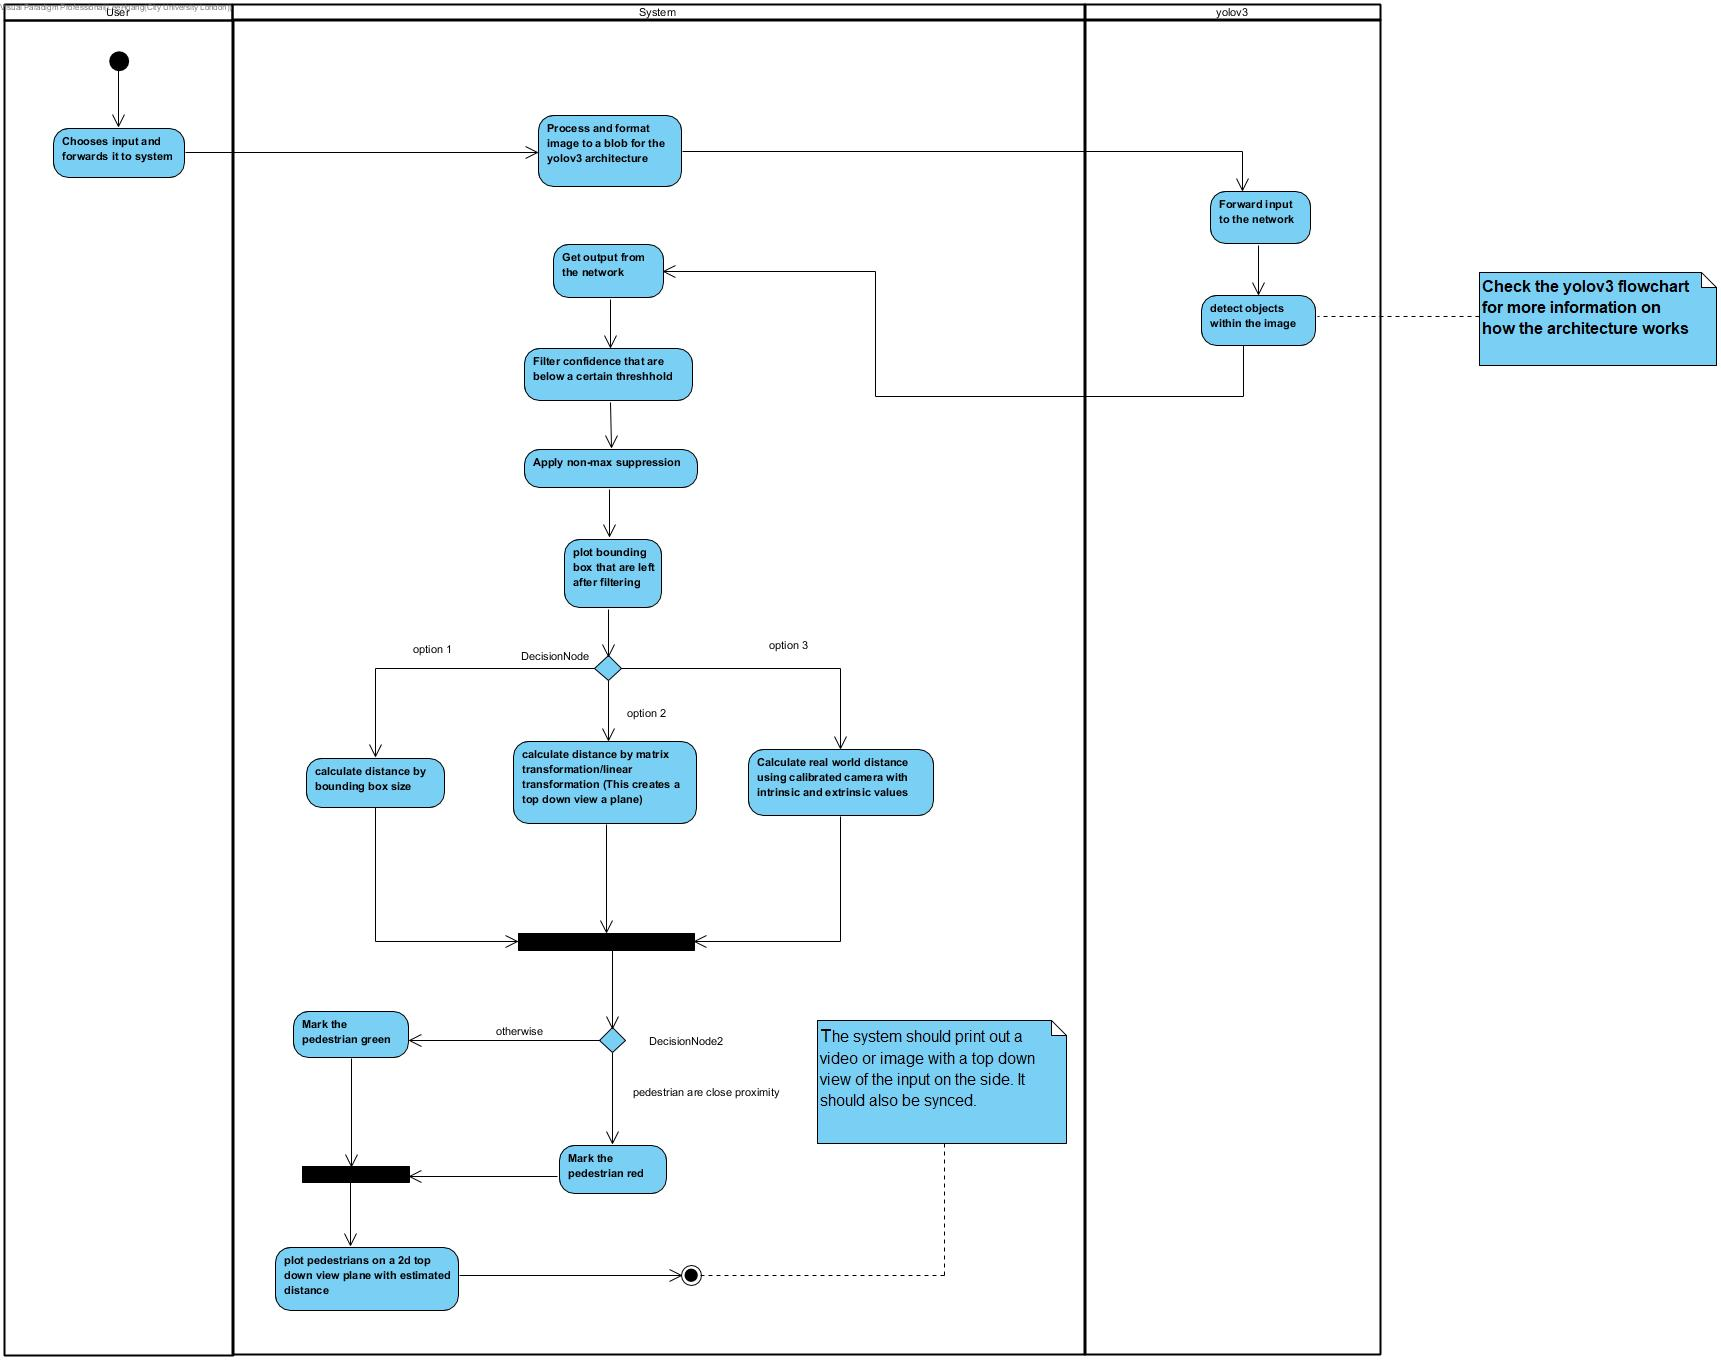
\includegraphics[width=170mm]{./images/system design.jpg}
	{Figure 4.2: Activity diagram describing the system pipeline}
	
\end{centering}

\vspace{10mm}

A class diagram (appendix 3) was created to show the functions that occur through out the system with the inputs and outputs. Each function also includes the key parameters needed, as well as the function's data type.

\section{Development phases}

The project has several development phases to give time to thoroughly test each feature of the system. These phases will be done in chronological order and will each be treated as a sprint.

\subsection*{Object detection with YOLO}

This phase will focus on forwarding images to the network to test how well the object detection works. The images used in the testing will have different density of population in the image, where some images will contain people overlapping another. The same images will also be artificially augmented by adding noise to image to limit test the architecture. This phase will also be testing videos as inputs, the main measurement of success will be how smooth each individual is tracked through out the processing.

\subsection*{Detecting social distancing by bounding box distance}

By using the found bounding box in the first phase, the program should be able to compute the distance between two people using pixels as a estimated measurement. Different linear scalars will be applied to the coordinates, solving the issue of perception.

\subsection*{Detecting social distancing by matrix transformation}

This method can be achieved by using the OpenCV library to calculate a matrix that transforms a quadrilateral in an image that is marked with 4 points to a square/rectangle image. this transformation is a combination of rotation, translation and shears. This will be tested with videos before and after distortion.

\subsection*{Detecting social distancing by camera calibration}

The dataset provides intrinsic and extrinsic values for the cameras used. This enables the project to convert pixel values to real world measurements, acquiring a very accurate solution to the problem. Using this method sucessfully will showcase how effective the other methods in comparison to each other.

\subsection*{Plotting pedestrians on a top down view of the image}

The system will create a side panel showcasing a top-down view of the pedestrians and if they are social distancing with a green or red highlight. This can be used to compared the social distancing detection methods.

\subsection*{Identifying groups of people and marking them 'safe'}

An algorithm will be developed to detect groups of people within a video. The system should be able to identify each person with their own key number in every frame. The motivation for this implementation is to allow parents and children to still maintain close contact and still be marked as social distancing.

\chapter{Results}

This section discusses the results found throughout the project.

\section{Detecting objects with 'yolov3' (Analysis)}

OpenCV enabled the use of 'yolov3' with the built-in functions of loading the weights of the neural network and forwarding an image to output the objects detected. 

\vspace{2mm}

The first image that was forwarded was 'image 2' (figure 5.1). The focus of using this specific image was to look at how well the model detected people who were overlapping each other. The outcome of model was over 5,000 objects detected within the image, taking 0.54 seconds to compute. The amount of objects detected might seem unnecessary, but the model was trained to detect 80 different objects, therefore will provide a large number of classifications per image.

\vspace{2mm}

Each bounding box that the model outputted produces several probabilities that the object detected is the correct classification. Therefore objects that are a 'person' will also have a probability of being identified as a 'car'.

\subsection{Filtering classification methods}

The probabilities can be filtered by extracting the highest probability that the model gave to an object within the image by using the argmax function that NumPy provides. This method of filtering removes 98.75 percent of the objects identified by YOLO. Since the model is trained to identify over 80 different classifications, there is only 71 objects detected when filtering 'person' from 'image 2'.

\vspace{2mm}

Another method of filtering was to apply a probability threshold (Confidence). Increasing the threshold filtrates all probabilities that are below a certain percentage. Figure 5.1 shows a plot that focuses on the number of objects that are detected with different levels of confidence with a 2 percent increment. Having a really high percentage means that model almost guarantees the object classification if correct. This has the draw back of not being able to detect any pedestrians far in the background (Appendix 4a), as they have lower classification percentage that the people closer to the camera. It is more optimal to have a lower percentage in 'image 2' as the system is able to pick up people who are hiding behind others even though they are close to the front of the camera which is important in an office environment.

\begin{center}
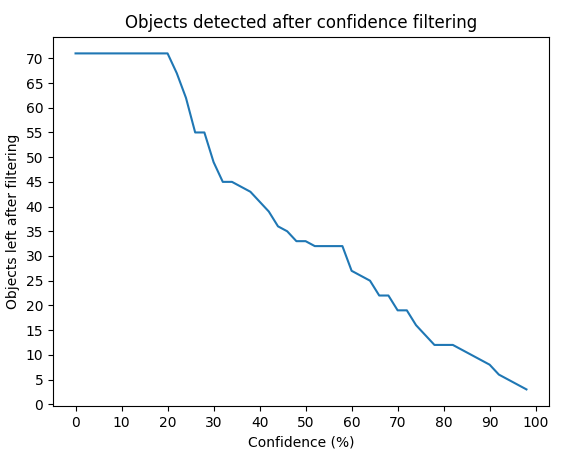
\includegraphics[width=75mm]{./images/appendix/ConfidencePlot.PNG}
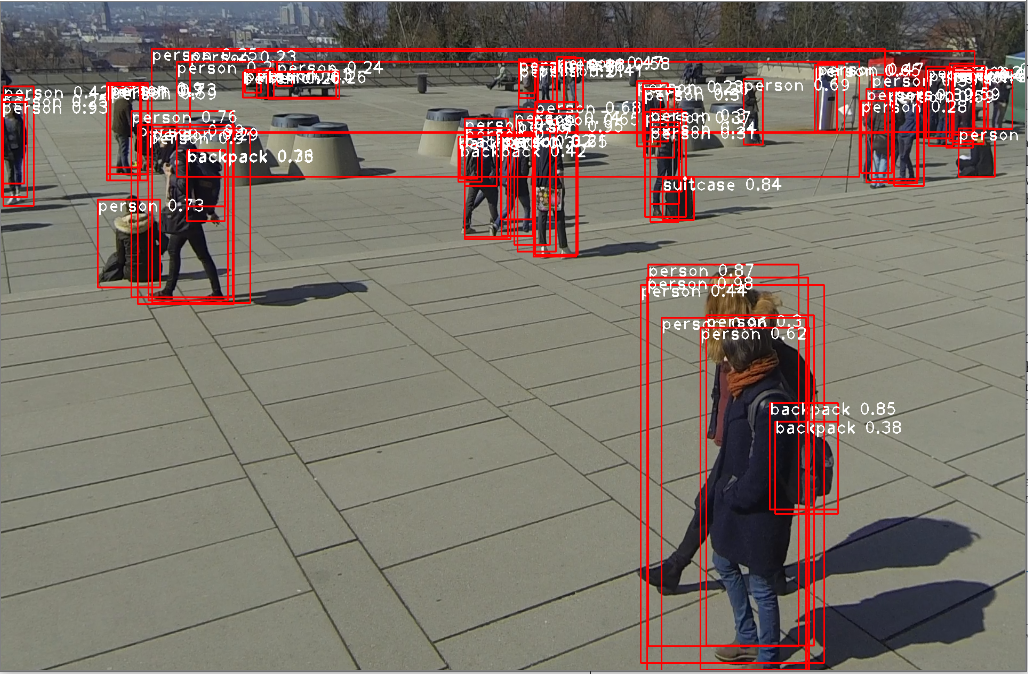
\includegraphics[width=75mm]{./images/zeroConfidence.PNG}

\vspace{3mm}
{\footnotesize Figure 5.1: Confidence plot on 'image 2' (left) and 'image 2' with 0 percent confidence (right)}
\end{center}

\subsection*{Non-max suppression}

The choice of having a small confidence has a clear down side of an increased amount of overlapping bounding boxes on the same object (Figure 5.1). To reduce the overlaps, the system uses non-max suppression which was discussed in the method section.  

\vspace{2mm}

Non-max suppression (NMS) has a parameter that can be tuned to either increase or decrease the effectiveness of NMS where a smaller parameter filters more bounding boxes on the same object. The function was testing with 'image 2' with a 30 percent confidence.

\vspace{2mm}

Contrary to the confidence parameter, having an extremely low parameter for NMS loses too much information in the process. Using 0.1 as the parameter with 'image 2', the person who is hiding behind the other in front of the camera view is not being detected in the finished output and majority of people in the background lost their bounding boxes. Losing the people in the background is less problematic if the system were to be used in an small office space, but, having a low parameter could harm the people who are hiding behind others as they will not be considered when calculating the social distancing. In this image, the person in front would be marked as 'safe' when calculating social distancing.

\vspace{2mm}

On the other hand, having a larger parameter value will keep too much information as there will be still be overlapping bounding boxes on the same object, not making full use of NMS. The reason why overlapping bounding boxes are bad for the final output of object detection is that when calculating if the person is social distancing, they will be seen as 'unsafe' even if there is no visible person next to them as the system relies on the position of the bounding boxes when calculating distance.

\vspace{2mm}

While there is a parameter value that voids all overlapping boxes and detects the person hiding behind the other in 'image 2' (value 0.6), the bounding box that NMS chose was suboptimal and is bigger than the person's body (Appendix 4b). Solving the problem by adjusting the 'yolov3' architecture can be difficult as the image itself was intentionally used as an extreme example and may even take humans a second to see that there is a person behind the other as there is finite detail of the person's body.

\vspace{2mm}

A higher camera angle when taking this picture could be a solution for hidden people, allowing for more exposure on the person's figure. Likely, a perfect angle for detecting people with this architecture would be close to a top-down view of the floor which acts as a planar surface, allowing to see every single person in view without the worry of hiding behind someone else. Achieving a fully working object detection on 'image 2'
 goes beyond what is currently capable of the YOLO architecture. Moving forward, any frames within a video that experiences the same level of object interference will be seen as an 'outlier' frame for simplicity. 

\subsection{Image augmentation}

The purpose of testing object detection with images that are augmented is that the inputs we are working with are high quality 1080p images and videos. It is possible that the user who wants to use the finished product have cameras that do not match the quality of the ones shown throughout the results.

\vspace{2mm}

This test will use 'image 4' for a baseline example and will be augmented, mainly focusing on the two people who are next to each other on the left (Figure 5.2). The image was reduced to 1280x720 resolution. All variations of the image was processed with a confidence percentage of 50 and 0.5 for the NMS parameter. 

\vspace{2mm}

The images will have artificial noise added using a technique called 'salt and pepper' (adding black and white pixels to random spots). The amount of 'salt and pepper' that is added to an image can be controlled by a parameter that determines the probability that a pixel in the image will either turn black/white or stay the same where turning black and white are same probability. This technique is done manually using a 'for' loop where the loop goes through every pixel of the image. A number is rolled each time within the for loop and is not set, this means that running the program again with the same parameters may lead to different results.

\vspace{2mm}

The first test using a 10 percent probability produced similar bounding boxes to the original image, with a slight difference of bounding box height/width and the probability of 'correct classification' also varied. While it is only a sample of one, 'yolov3' seems to work well with different resolutions and noise which is shown in figure 5.2, successfully identifying the two people who are on the left.

\vspace{2mm}

When increasing the intensity of noise, the bounding boxes that are shown decreases in quantity as the model is having a harder time determining the probability that the object is a 'person'. Augmenting the image to 50 percent noise (figure 5.2) made it so the object detector could not identify a 'person' with above 50 percent confidence. 

\vspace{2mm}

With a 0 percent confidence and without NMS (Appendix 4c), all variations of the augmented images do identify the two people. This concludes that not having a high quality image may affect the probability that the system correctly classifies an object, but can be solved by lowering the confidence threshold. The drawback of having a lower quality camera is that it reduces the total number of bounding boxes which may lead to people being unidentified by the system.


\begin{center}
	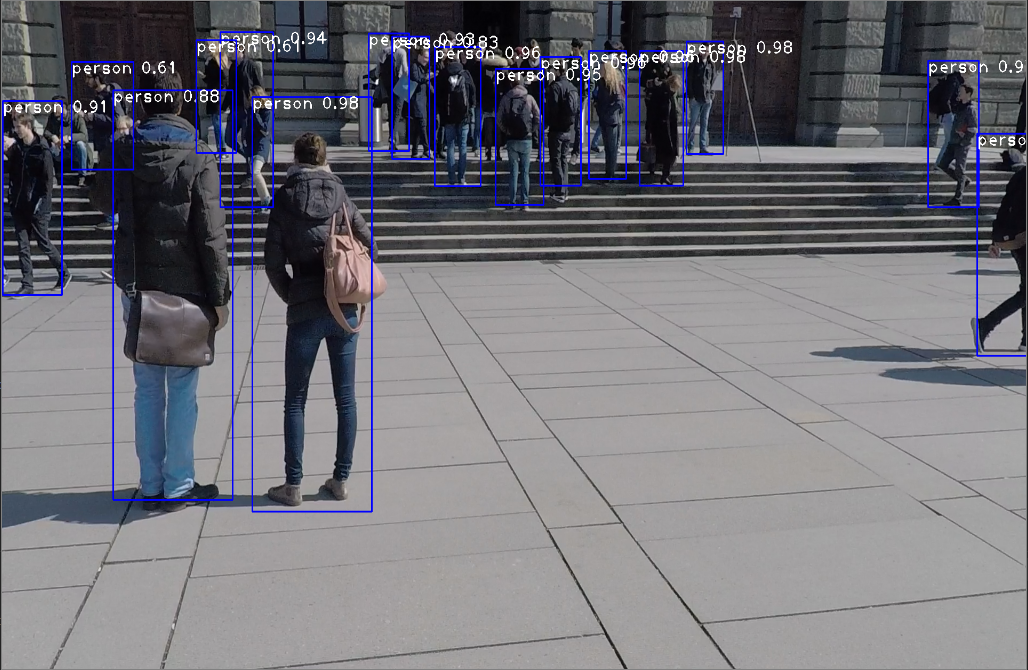
\includegraphics[width=65mm]{./images/image45050.PNG}
	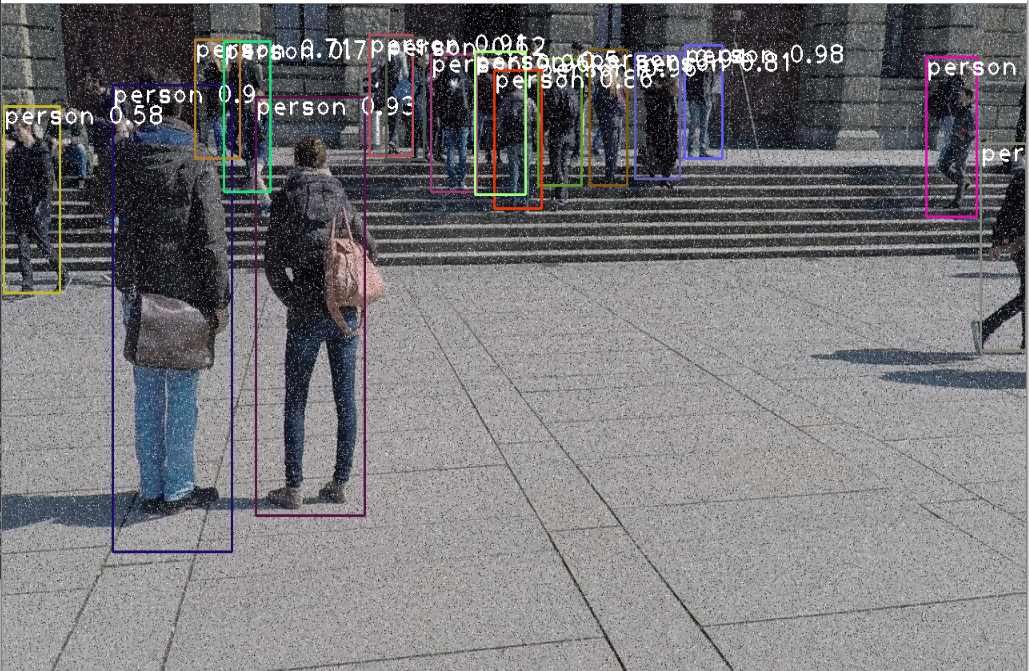
\includegraphics[width=65mm]{./images/appendix/imageAugment720pSandP.PNG}
	
	\vspace{2mm}
	\hspace{0.3mm}
	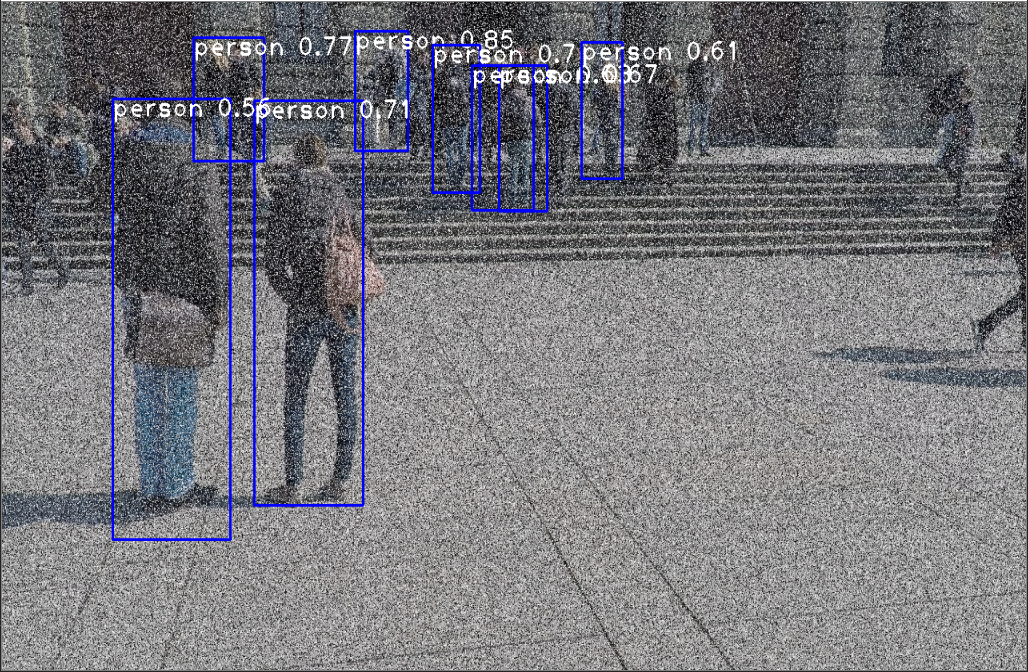
\includegraphics[width=65mm]{./images/appendix/imageAugment0.4SandP.PNG}
	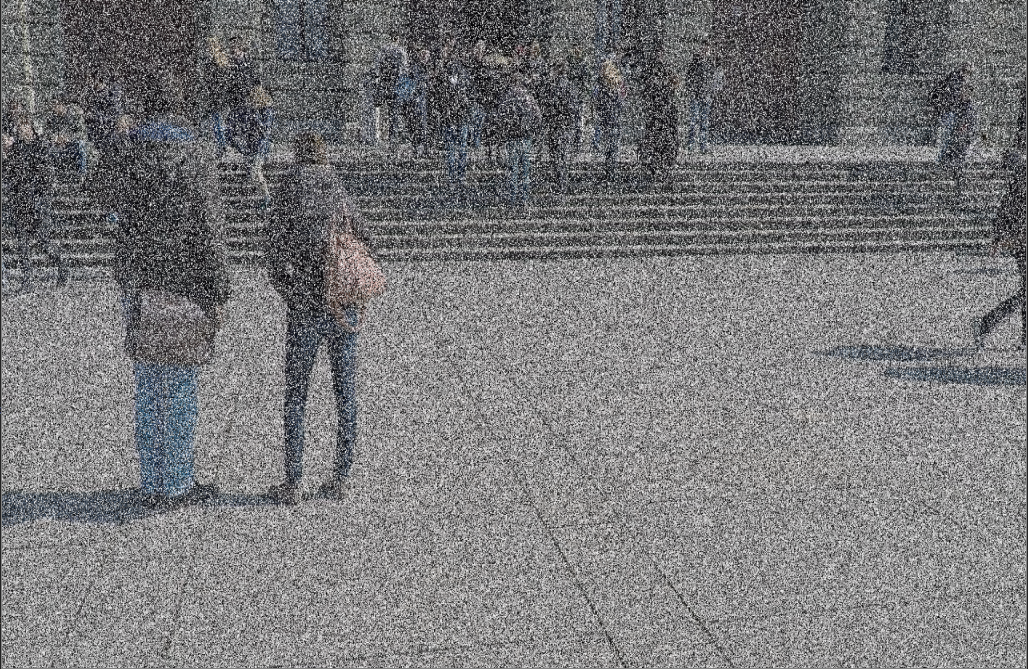
\includegraphics[width=65mm]{./images/appendix/imageAugment0.5SandP.PNG}
	\vspace{3mm}
	
	{\footnotesize Figure 5.2: 'Image 4' with artificial noise of 0,10,40,50 percent respectively}
\end{center}


\subsection{Conclusion for detecting objects}

The architecture worked well for all images that were tested but have limitations that can occur when an object blocks another. However, having a better camera angle will solve the issue and is recommended when using this system. Tuning the confidence and NMS effectiveness can be finicky and can differ depending on the camera quality used therefore testing different parameter values for the user's setup before using the system for surveillance is essential to avoid miscalculation.

\section{Using a video as an input}

A while loop is used to read each frame of the video in chronological order and is fed to the model. With the help of GPUs, the process of forwarding each frame to the network is sped up by roughly 4 times compared to using a CPU only. See appendix 5 for screenshots of 'video 3'

\vspace{2mm}

Beneficiaries are able to use their webcam/surveillance cameras as an input in real time with this implementation. The downside of running this program in real time with a camera of 30 frames per second is that it requires more GPU power compared to the results seen in the report. Currently the setup in this report computes the videos at approximately 10 frames per second. 

\section{Detecting social distancing by bounding box}

Using the bounding boxes that 'yolov3' architecture has identified, the system in theory should be able to mark the middle of every 'person' in the image/video. To calculate the middle of bounding box coordinates, the model provides the position of the left-upper corner of the bound box represented as (x,y) and also gives the height and width of the bounding box as h and w respectively. Therefore:
\begin{equation*}
Middle Of Bounding Box Coordinates = (x+\frac{w}{2}, y+\frac{h}{2})
\end{equation*}


To calculate distance between every individual using the bounding boxes given, the system uses a 'for' loop of time complexity O($n^2$) to draw a line between every individual in the image/frame. The line can be measured using Pythagoras' theorem. Once calculated, the system filters lines that are below the social distancing threshold red, else the line is green. For the results produced, some green lines were filtered if they were larger than a certain threshold to give better clarity on the lines that showed 'not social distancing'. See appendix 6a for an example of all the lines in a single image.

\vspace{2mm}

For the first prototype of the system, the threshold of social distancing is measured by pixels. The first test uses 'image 4' with the threshold of 400 pixels being the social distancing length. This length was determined by measuring the two people who are next to each other with pixels (approximately 360 pixels apart) and slightly increasing the number. This also means that images from different cameras will need different threshold values due to the angle of the camera and the camera's focal length.

\vspace{2mm}

The results seen in figure 5.3 do correctly identify the two people as not social distancing between each other, but there are connections from the two people at the front to people at the back who are seen by the system as not social distancing when in reality they are far away. This is because the current system does not consider perception, therefore the image plane acts a top-down view of the real world instead of looking a plane at an inclined angle.

\vspace{2mm}

This is not the only problem with the system as measuring distance at the middle of the bounding box with the y coordinate has inaccuracies as doing so assumes that every person in the photo is the same/average height which is not the case. A better solution for this is to view the ground as a planar surface, and use the bottom of the bounding boxes or person's feet as a mark/coordinate point when measuring distance. 

\begin{center}
	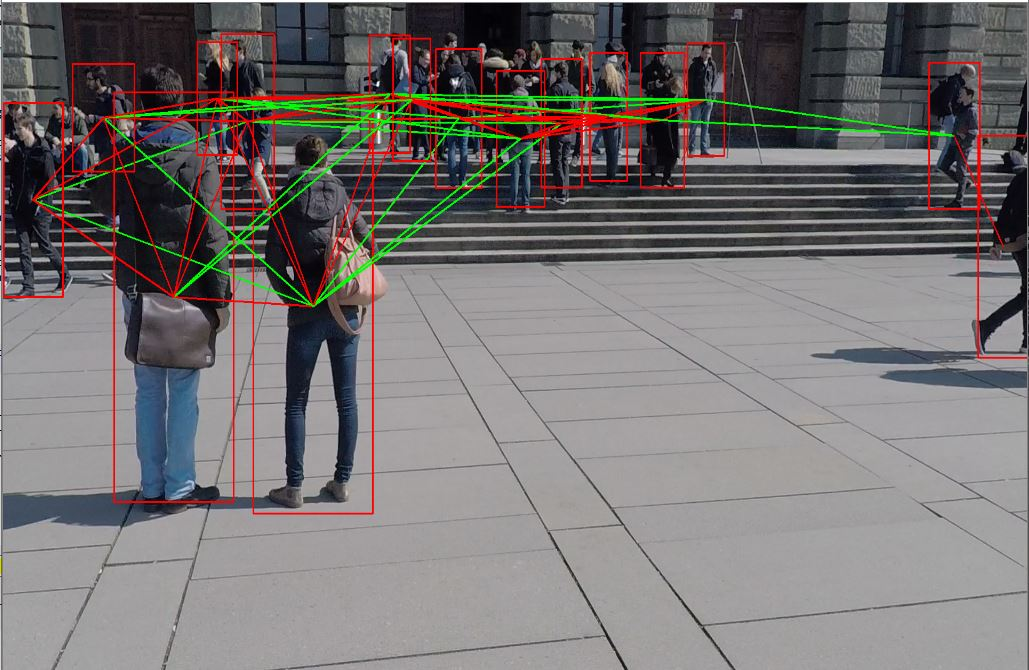
\includegraphics[width=65mm]{./images/appendix/test1.JPG}
	
	{\footnotesize Figure 5.3: 'Image 4' with first prototype social distancing detection}
\end{center}

\subsection*{Bounding box measurement improvement}

The first improvement to the system was to change the coordinates of where the line was being measured. Instead of using half of the bounding boxes' height added to the y coordinate, the system adds 99 percent of the height. 99 was specifically used because the bounding boxes generated by the model could sometimes overshoot the person's shoe, therefore using slightly less than the bounding box height would correct this. 

\vspace{2mm}

While the improvement to the system did not classify anyone people as 'social distancing', the connections coming out of the two people at the front and the people in the background  (Figure 5.4) are green, indicating that they are a safe enough distance. This improvement provides flexibility between the images/videos used in the dataset (See Appendix 6b for results on 'video 9'), as the implementation does not need to be tweaked when changing cameras. 

\begin{center}
	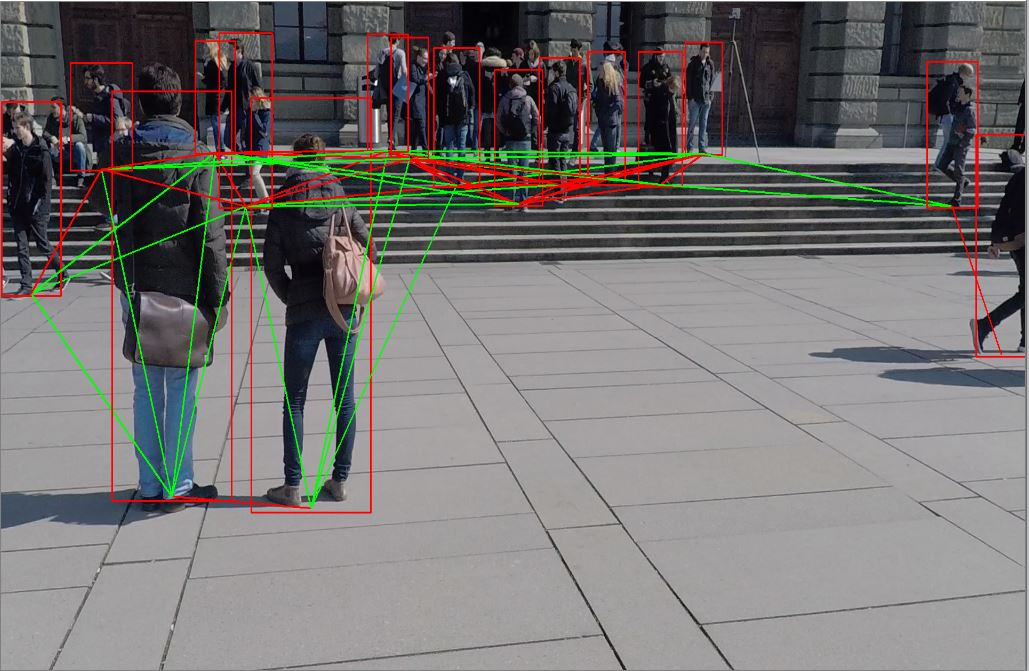
\includegraphics[width=80mm]{./images/appendix/BoundingBoxBottom.JPG}
	
	{\footnotesize Figure 5.4: 'Image 4' with measurement improvement.}
\end{center}

\subsection*{Solution to perspective distance}

Looking at the tiles of the floor in 'image 4', the tiles get smaller as they get further from the camera linearly. The rate at which they get smaller depends on several factors: the focal length of the camera and the distance from the camera. The equation to calculating the size of a person in the image respective to how far they are from the camera would be:

\begin{equation*}
Object Size In Image = Object Size * \frac{Focal Length}{Object Distance From Camera}
\end{equation*}

The implementation of this method will only rely on pixel distance between two bounding boxes, therefore we can not use the actual focal length of the camera and object distance from camera as parameters in the equation. Therefore a solution to this is to use the x and y coordinate of the bounding boxes to determine how far the person is from the camera, where the smaller the y, the further the object is from the camera. (the coordinate (0,0) starts at the top left-hand corner of the image.)

\vspace{2mm}

The first solution was to multiply every y coordinate by 2 while keeping the threshold the same (400 pixel distance). This in theory is the focal length parameter as an estimate and also could be seen as a stretch in the x axis. People who are on the same y coordinate are in the same perspective distance, therefore multiplying the y coordinate will have very little effect on people who have the same y value when calculating Pythagoras where as people who are on different y coordinates with be impacted greatly. 

\vspace{2mm}

The results (Figure 5.5) show a large improvement to the previous version, being able to classify 3 different people as 'social distancing' unlike figure 5.4. The implementation still classified the two people at the front as not 'social distancing' which is a success.

\begin{center}
	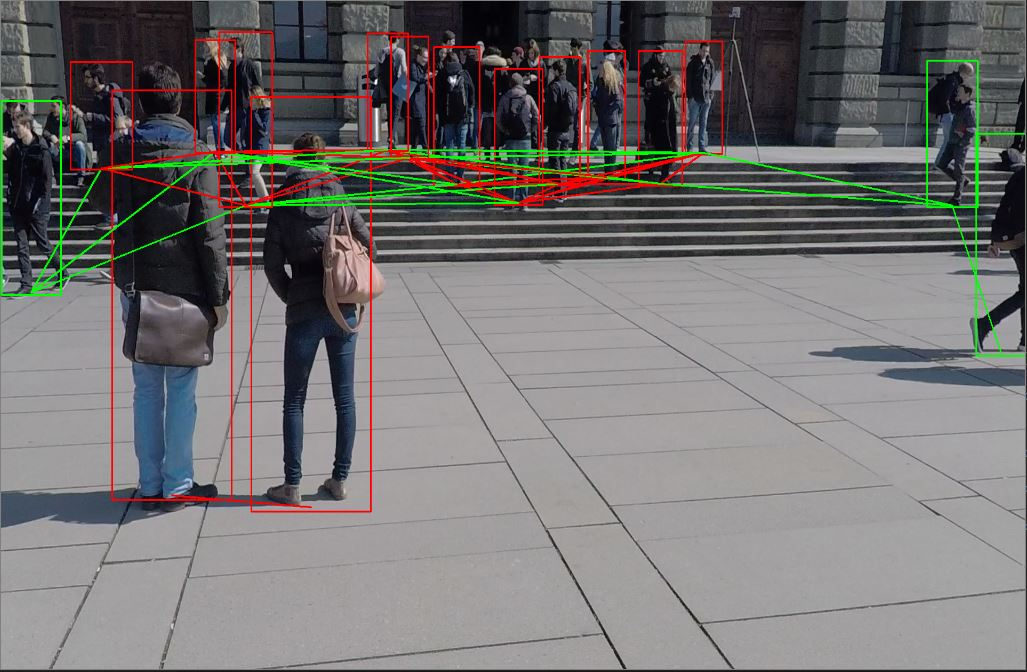
\includegraphics[width=80mm]{./images/appendix/PerspectiveSolution1.JPG}
	
	{\footnotesize Figure 5.5: 'Image 4' with measurement improvement.}
\end{center}

While this is an improvement, the perspective is only 'solved' in the y axis. As things are further away from the camera or the y coordinate becomes smaller, each pixel represents a larger area in the real world. Therefore the system would need to scale the threshold depending on the value of the y coordinate. The equation used to calculate the new threshold with respect to the y coordinate is:

\begin{equation*}
UpdatedThreshold = OriginalThreshold - \frac{OriginalY*Scalar}{MeanCoordinateBetweenObjects}
\end{equation*}

The 'OriginalY' variable is based of the y coordinates of where the 'OrginalThreshold' was measured (This can be referred from the first prototype of the implementation.). In 'Image 4' case, the 'OriginalY' is the mean y coordinate between the two people at the front (value 800). 

\vspace{2mm}

Figure 5.6 showcases the before and after of the 'threshold scalar' implementation using the different 'scalar' value at 20, 40, 50 respectively. The turquoise lines indicate not 'social distancing' between people. While  the implementation does not classify anyone new as being 'social distancing' with the 'scalar' value being 20, some lines are removed between the two cluster of people in the background. The reductions of lines seen between the before and after indicate that the equation discussed previously is working as intended.

\vspace{2mm}

As the scalar increases, less and less connections appear in the final output of the image and more people are highlighted in green which means that they are 'social distancing'. With the 'scalar' variable being 50, only adjacent people are connect with lines. The method is very effective at dealing with perspective distance as the two people at the front are still classified as not 'social distancing'.

\begin{center}
	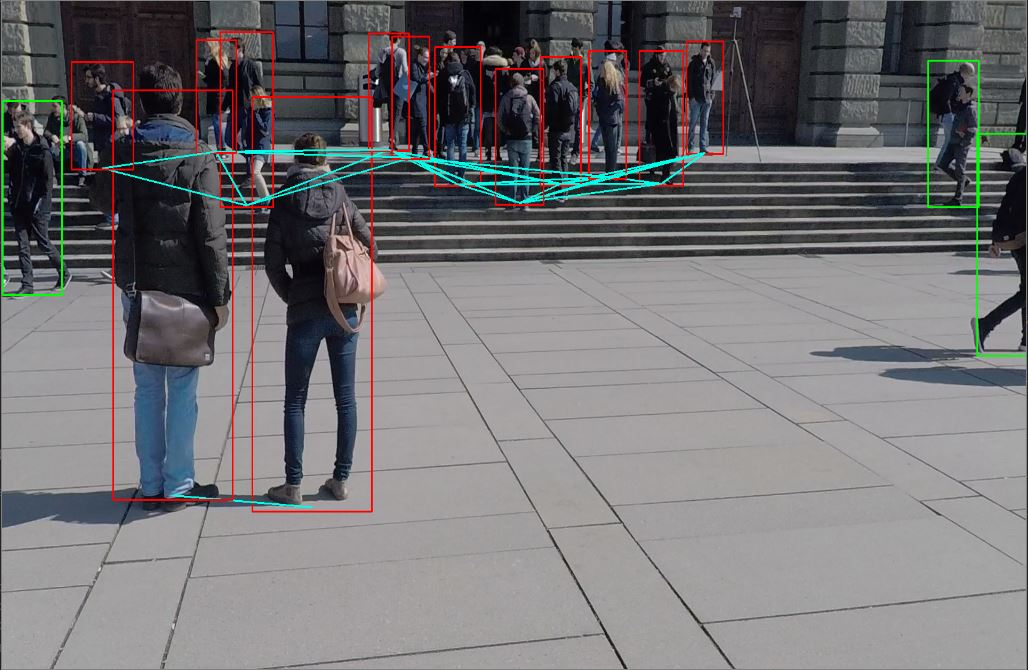
\includegraphics[width=65mm]{./images/appendix/BeforeThresholdScale.JPG}
	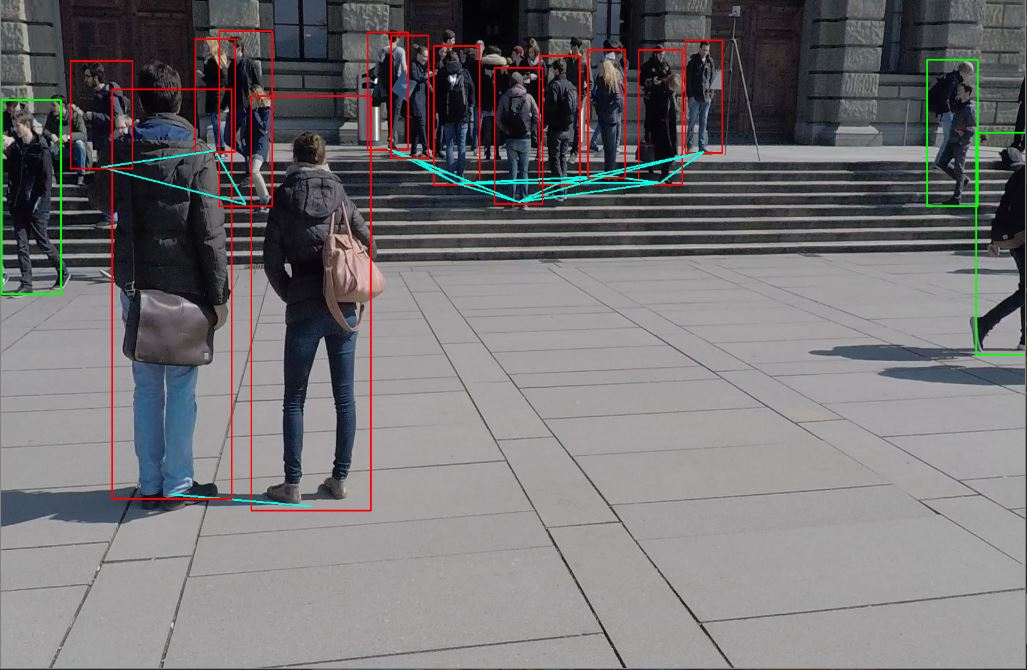
\includegraphics[width=65mm]{./images/appendix/AfterThresholdScale.JPG}
	
	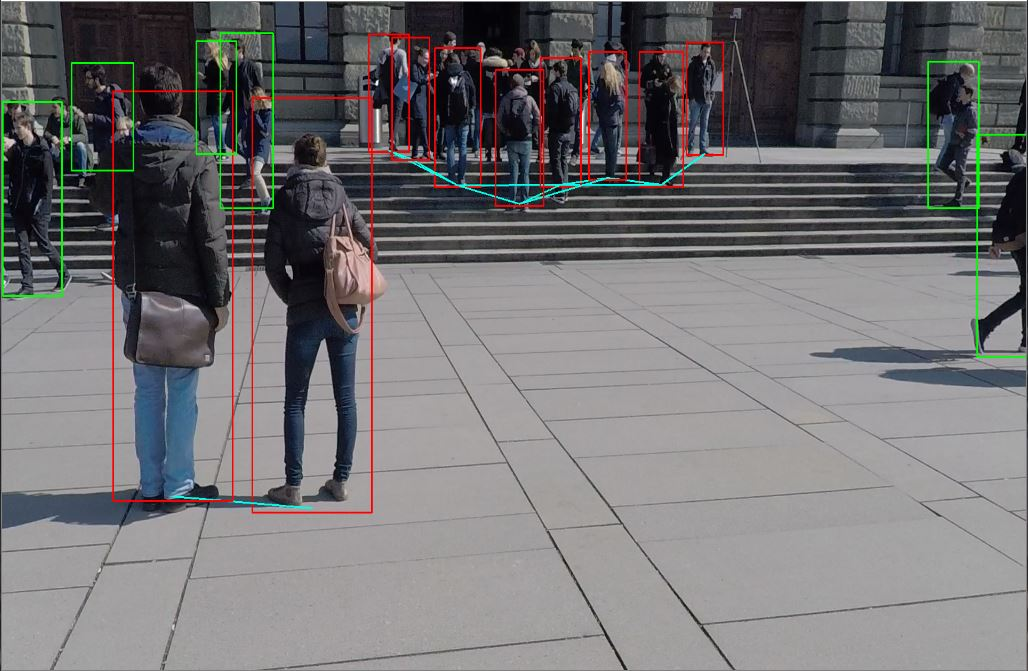
\includegraphics[width=65mm]{./images/appendix/AfterThresholdScale40.JPG}
	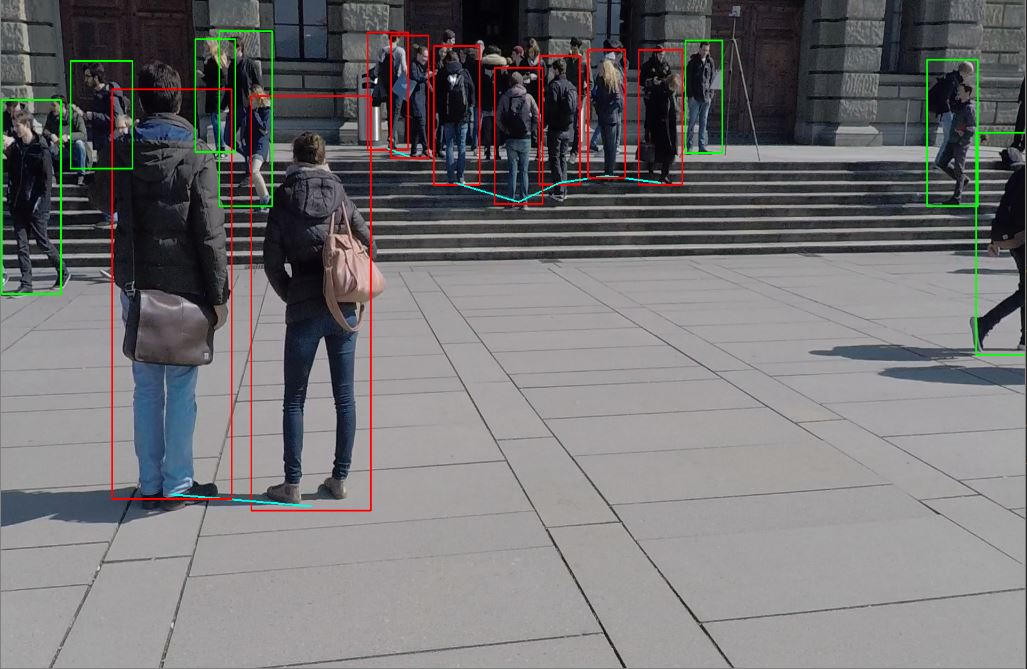
\includegraphics[width=65mm]{./images/appendix/AfterThresholdScale50.JPG}
	
	{\footnotesize Figure 5.6: 'Image 4' before and after scalar adjustments (Non,20,40,50 respectively).}
\end{center}

\subsection{Conclusion of detecting SD by bounding box}

The final output of the method worked as intended. The combination of the two equations discussed could be seen as two separate transformation (stretch) to the image to account for the incline angle the camera has to the floor of the image.
\vspace{2mm}

The problems that this implementation has is that the measurements are pixel values and not real word value, therefore we cannot know the exact distance between each person. Solutions such as giving a single pixel a defined real world measurement is plausible by using the average measurements of an object in the image for scale with respective to a pixel, but the value will vary depending on the different focal lengths each camera has.

\vspace{2mm}

Another problem with this method is that the beneficiaries will have to tune the variables in the equation if they choose to use this for detecting social distancing. It is very likely that their setup is different and getting reasonable numbers for the variables will takes a lot of trial and error. 
In conclusion, this solution is only an estimate to calculating social distancing and is nowhere near perfect. 

\section{Detecting social distancing by matrix transformation}

The previous method uses the floor in the images/videos as a planar surface for better precision when calculating the final output. This method takes the same ideas and uses a matrix transformation to augment the image into a top-down view. The user selects 4 points in the image where each point is pointing towards the floor with an x and y component (Most likely the points connect to a irregular quadrilateral). The system is able to utilise a function from OpenCV called 'getPerspectiveTransform' which is able to calculate a 3x3 matrix that transforms the 4 connected points to another irregular quadrilateral or rectangle. The relationship between the plane selected and the image produced is called homography (OpenCV: Basic concepts of the homography explained with code, 2021) as they both represent the same planar surface in the real world.

\vspace{2mm}

Once the matrix is acquired, OpenCV has another function that transforms the image with the new found matrix from 'getPerspectiveTransform' by using the function 'warpPerspective'. Figure 5.7 features 'video 6' with a red quadrilateral draw on. The 4 corners in image coordinates (x,y) are the inputs to 'getPerspectiveTransform' with (150,222), (594,170), (2620,560), (370,1494) (top left, top right, bottom right, and bottom left respectively). Do note that the quadrilateral drawn is an estimate of a rectangular surface in the real world.

\begin{center}
	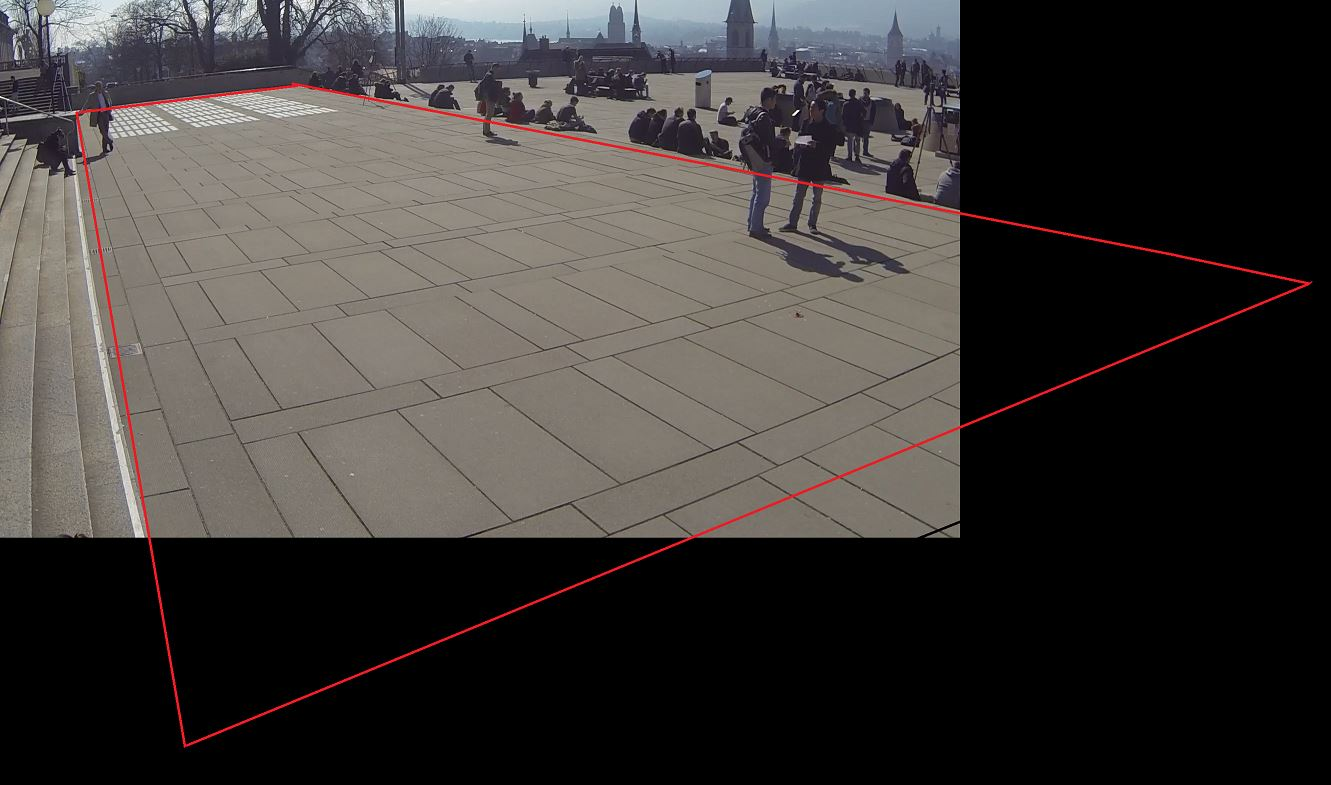
\includegraphics[width=80mm]{./images/appendix/QuadSelected.JPG}
	
	{\footnotesize Figure 5.7: 'Video 6' with the 4 connected coordinates.}
\end{center}

The image shown in figure 5.8 represents a concatenated image of both the before and after transformation. The concatenation was performed using a function that numPy provides. The image on the right in figure 5.8 tries to simulate a top-down view of the selected area in figure 5.7. 

\vspace{2mm}

With this function in place, the system can perform object detection on the original video and transform each interest point (which is the bottom of the bounding box discussed in the previous section) with the matrix M. Each interest point will be measured between each other, similar to the the previous method using Pythagoras. The equation of finding the transformed interest point (x',y') with the transformation matrix M where (x ,y) are the original points is:

\begin{equation*}
a
\begin{bmatrix}
x' \\
y' \\
1
\end{bmatrix}
=
\begin{bmatrix}
ax' \\
ay' \\
a
\end{bmatrix}
= M
\begin{bmatrix}
x \\
y \\
1
\end{bmatrix}
\end{equation*}

\begin{center}
	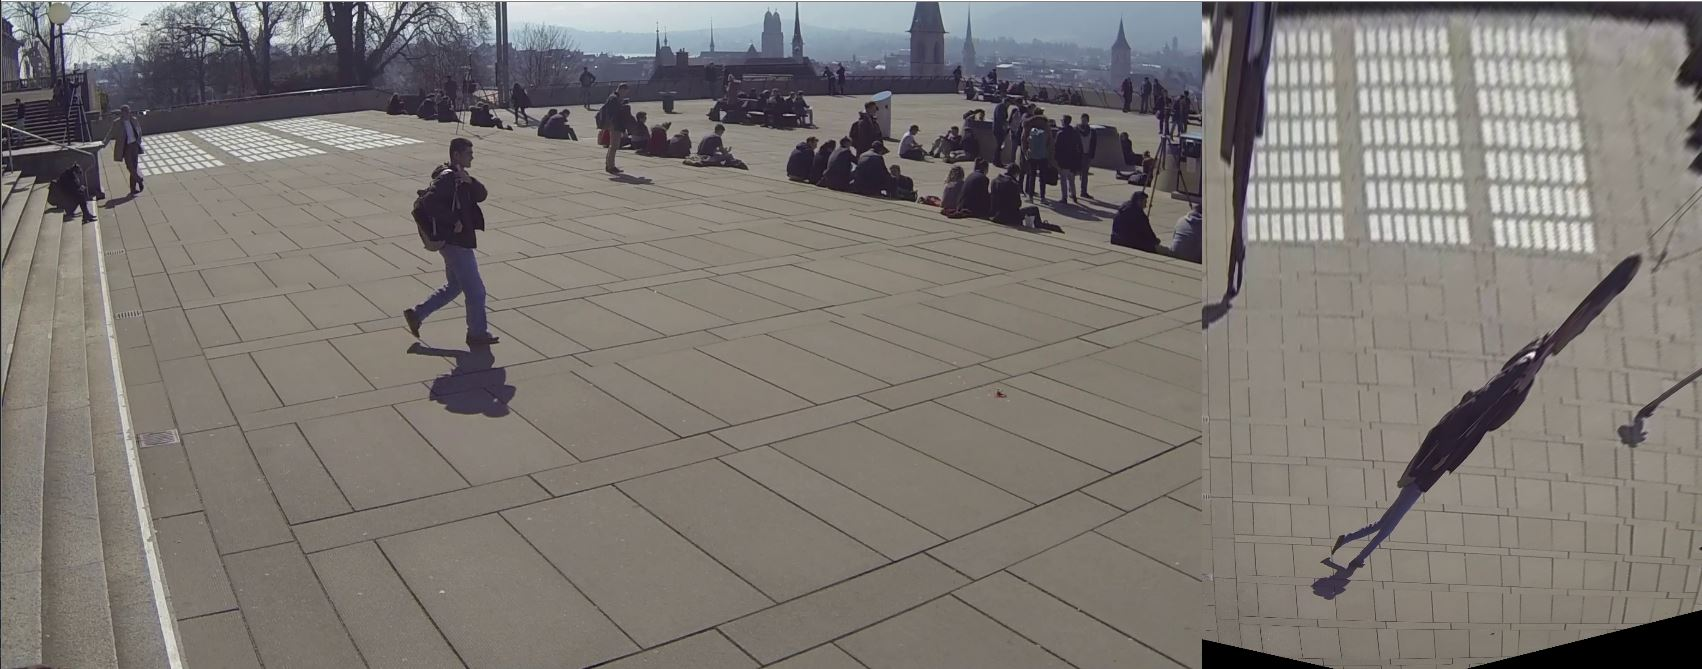
\includegraphics[width=120mm]{./images/appendix/ConcatenateImages.JPG}
	
	{\footnotesize Figure 5.8: 'Video 6' with the before and after transformation concatenated into one image.}
\end{center}

Figure 5.9 showcases the output of calculating social distancing after the transformation. Only people who are in the red box in figure 5.7 are used to calculate social distancing as the transformation only produces a top down view of that specific area. This is done by putting a threshold that filters out any interest point that were not in the red box after transformation. 

\vspace{2mm}

The threshold used in figure 5.9 to be not 'social distancing' is 400 pixels on the transform image. The threshold successfully identified the correct people as not 'social distancing' (people with red circles). Since the method tries to produce a top-down view of the plane select, the system is able to allocate a fixed real world distance to a single pixel if necessary. Appendix 7 shows more screenshots of matrix transformation with 'video 6'.


\begin{center}
	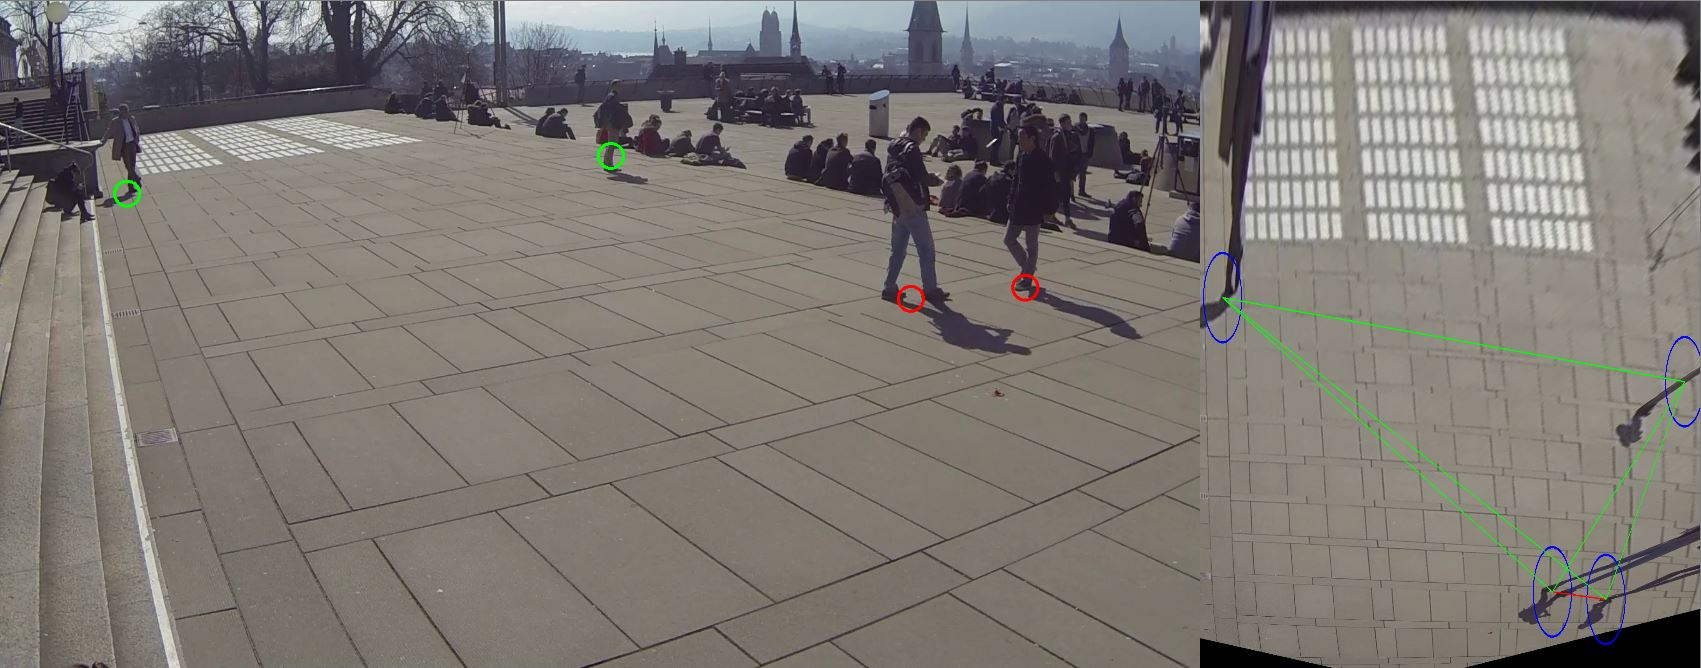
\includegraphics[width=130mm]{./images/appendix/MatrixTransExample3.JPG}
	
	{\footnotesize Figure 5.9: 'Video 6' with detecting social distancing with matrix transformation.}
\end{center}

\subsection{Conclusion of detecting SD by matrix transformation}

When comparing methods between the two discussed social distancing detectors, matrix transformation has the benefit of having easier and less parameters to tune. Matrix transformation only requires 4 points in the image as parameters compared to 5 parameters for the previous method. The beneficiaries also do not need to worry about trial and error for tuning the parameter for results that are only an estimate to calculating real world distances between people.

\vspace{2mm}

The downside to the matrix transformation is that it can only include people within the red box seen in figure 5.7 to be considered when calculating social distancing. This may be seen as a limiting factor for beneficiaries who have non-quadrilateral rooms for their offices. It is recommended to use a low focal length to get a better view of the area when using this method.

\vspace{2mm}

Another issue with this method is that it does not count for distortion within the images. This can be seen as very problematic when looking for accurate results. Looking at figure 5.7 and the right side of figure 5.8, there are curves in the images due to the distortion created by the camera. A way to combat this is to use calibrated cameras to find distortion coefficients (This is in the form of a 5 value vector) to account for non-linear errors in the image.

\vspace{2mm}

Figure 5.10 uses a function provided by OpenCV called 'undistort' to remove distortion in the image. The camera parameters needed for this function is the camera matrix which describe the mapping of a pinhole camera from 3D points in the world to 2d points in an image and distortion coefficients. This function is used before the 'yolov3' model detects any objects within the image.

\vspace{2mm}

The results of removing the distortion straightens the lines on floor in both the original and transformed images. The transform image can now be seen as a more accurate top down view image than before.

\begin{center}
	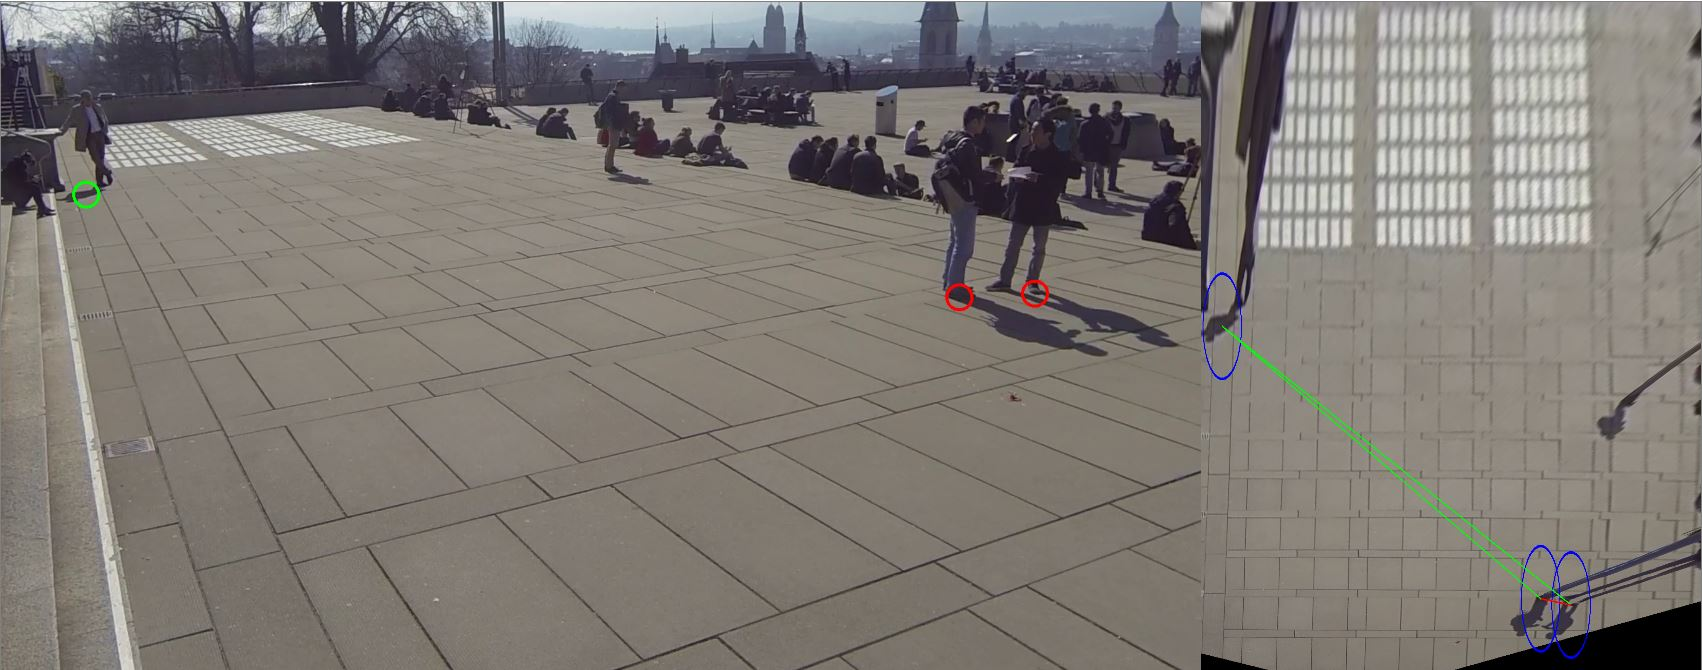
\includegraphics[width=130mm]{./images/appendix/UndistortedImageWithMatrixTransformation.JPG}
	
	{\footnotesize Figure 5.10: 'Video 6' with no distortion.}
\end{center}

Matrix transformation with distortion coefficients is very suited for commercial uses and can be seen used in other social distancing detectors (Y. C. Hou, 2020). The paper uses the same method but without using distortion coefficients, producing less accurate results.

\section{Detecting SD by calibrated camera.}

Camera calibration is the process of acquiring intrinsic and extrinsic values of the camera. The extrinsic parameter describes the location of the camera in the real world, usually described by both a rotation matrix/vector and a translation vector. Normally the origin of the coordinates is with respect to camera's focal points. The WILDTRACK dataset feature multiple static cameras, therefore they share a single origin which is not directly pointing at any of the cameras.

\vspace{2mm}

The intrinsic parameters holds the values of the focal length and principle point of the camera in a single matrix which is regularly called the 'camera matrix' as well as holding the distortion coefficients. The camera matrix maps the scene in front of the camera to pixel coordinates.
\vspace{2mm}

With the combination of both the intrinsic and extrinsic parameters, the equation to map real world coordinates to an image plane is (Robert Collins):

\begin{equation*}
\begin{bmatrix}
x \\
y \\
1
\end{bmatrix}
=
\begin{bmatrix}
f_{x} & 0 & c_{x} \\
0 & f_{y} & c_{y} \\
0 & 0 & 1
\end{bmatrix}
\begin{bmatrix}
r_{11} & r_{12} & r_{13} & t_{1}\\
r_{21} & r_{22} & r_{23} & t_{2}\\
r_{31} & r_{32} & r_{33} & t_{3}
\end{bmatrix}
\begin{bmatrix}
X \\
Y \\
Z \\
1
\end{bmatrix}
\end{equation*}

or an abbreviated version:
\begin{equation*}
\begin{bmatrix}
x \\
y \\
1
\end{bmatrix}
= ^{c}M[R \ |\ T]
\begin{bmatrix}
X \\
Y \\
Z \\
1
\end{bmatrix}
\end{equation*}


There are multiple algorithms to calibrate a camera (Remondino et al. 2005). The WILDTRACK dataset uses the pinhole model to calibrate their cameras (Wikipedia [2017b]). Do note that this type of camera calibration only produces a near estimate of the parameters but is very close. Appendix 8a is an illustration of how the cameras overlap in view made by the creators of the WILDTRACK dataset and also a plot of the cameras using MATLAB in appendix 8b.

\vspace{2mm}

The biggest problem with transforming 3d points in space to a 2d point in an image plane is that there is a lot of information lost in the process, essentially losing the Z axis. Therefore reversing the process can prove troublesome if the camera calibration is done incorrectly.

\vspace{2mm}

One of the ways beneficiaries can transform 2d image points to 3d image points using the intrinsic and extrinsic parameters is to calibrate the camera so that the floor is at 0 with the z-axis with respect to the camera. Acquiring these extrinsic parameters, we can use the inverses of the intrinsic and extrinsic parameters (multiplied together creates a homography matrix) with this equation where u,v are image coordinates and X,Y are 3d coordinates :

\begin{equation*}
\begin{bmatrix}
X \\
Y \\
1
\end{bmatrix}
=
\begin{bmatrix}
f_{x} & 0 & c_{x} \\
0 & f_{y} & c_{y} \\
0 & 0 & 1
\end{bmatrix}
^{-1}
\begin{bmatrix}
r_{11} & r_{12} & t_{1}\\
r_{21} & r_{22} & t_{2}\\
r_{31} & r_{32} & t_{3}
\end{bmatrix}
^{-1}
\begin{bmatrix}
u \\
v \\
1
\end{bmatrix}
=
\begin{bmatrix}
h_{11} & h_{12} & h_{13}\\
h_{21} & h_{22} & h_{23}\\
h_{31} & h_{32} & h_{33}
\end{bmatrix}
^{-1}
\begin{bmatrix}
u \\
v \\
1
\end{bmatrix}
\end{equation*}

While the camera calibrations in the WILDTRACK dataset are not calibrated specifically for this equation, the method was still attempted to see if the system could produce a good estimate of the person's position which can then be used measure social distancing.

\vspace{2mm}

The method was tested on the same person using 2 different cameras (the first frame of both camera 1 and camera 6). The extrinsic parameters that the WILDTRACK dataset provides is both a rotation vector and translation vector. As we need a rotation matrix, OpenCV provides a function called cv2.Rodrigues that outputs a rotation matrix with an input of a rotation vector and vice versa.

\vspace{2mm}

The x,y output of the same person with different cameras were mismatched which was expected as the cameras were not calibrated to allow for the floor to be 0 in the Z-axis. In terms of producing a good estimate of where each person in the frame were with respective to each other was good, the vector output seemed to be surprisingly well done. Figure 5.11 showcases each person in 'video 8'  who is being detected to have their bounding box coordinates transformed by the formula above and be plotted on a graph. When paying close attention to the groups of dots in the plot, it represents a good estimation of where the respective groups are in the real world.

\vspace{2mm}

This ultimately means that this method is feasible for calculating social distancing. So the next step that was taken is applying Pythagoras' theorem to calculate the distance between each person and apply a threshold to mark people as 'social distancing'.



\begin{center}
	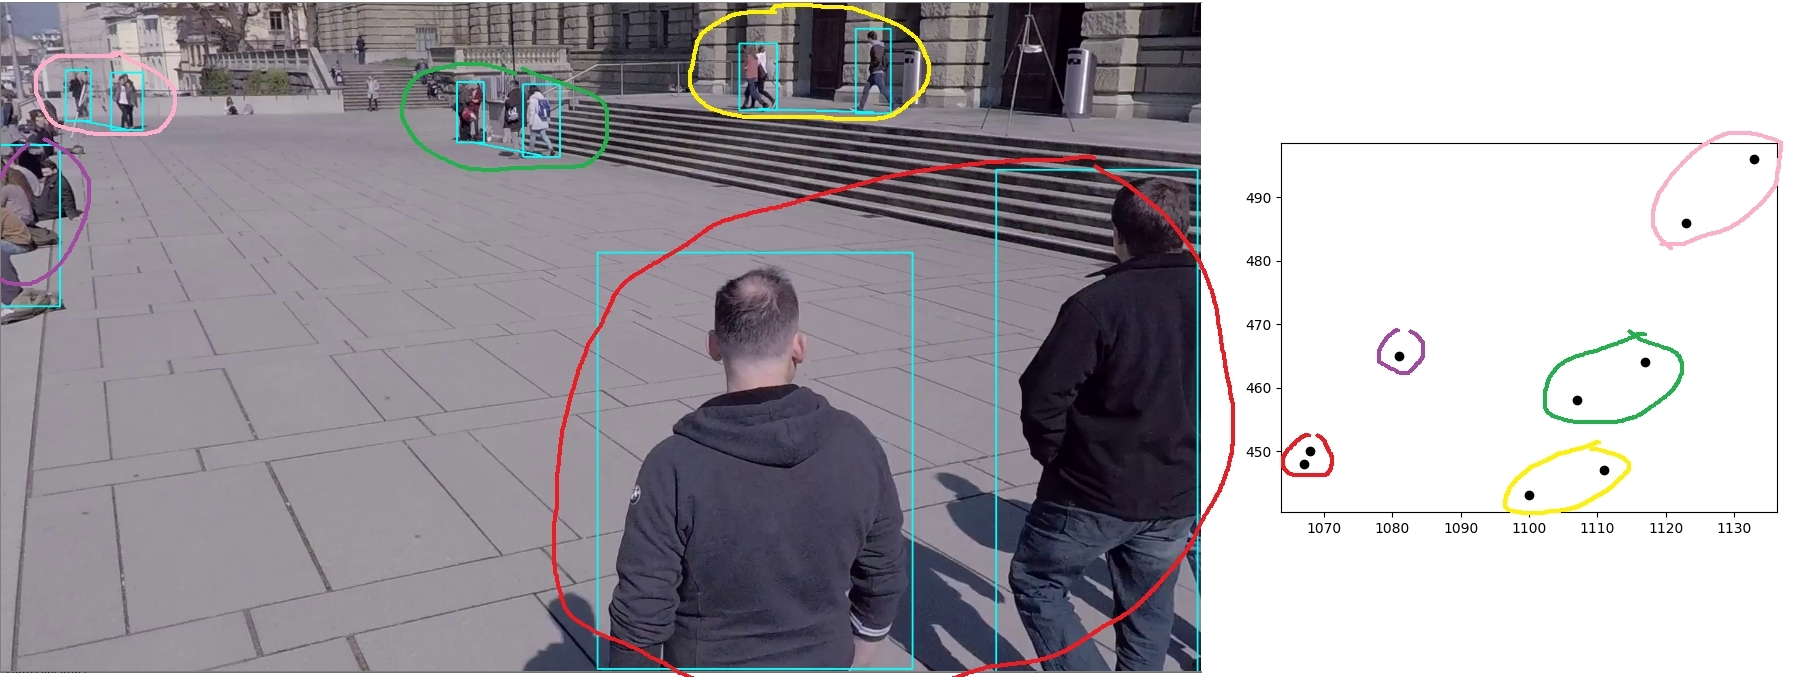
\includegraphics[width=150mm]{./images/appendix/HomographyMapping.JPG}
	
	
	{\footnotesize Figure 5.11: 'video 8' with homography transformation.}
\end{center}

The implementation was carried through similar to the matrix transformation section which was using a static threshold to detect people who were not 'social distancing'. Figure 5.12 displays two different frames of 'video 8' with the implementation.

\vspace{2mm}

While the transformation output has no relevance to the actual real world coordinates of the people, the output could be seen as pseudo real world coordinates that are only relevant to the camera output alone. Since we are working with pseudo real world coordinates, the threshold used in figure 5.12 was less than 5 units unlike the previous examples where the threshold was 3 digits minimum. The overall output worked well, being able to identify clusters of people as not 'social distancing' whenever applicable.

\begin{center}
	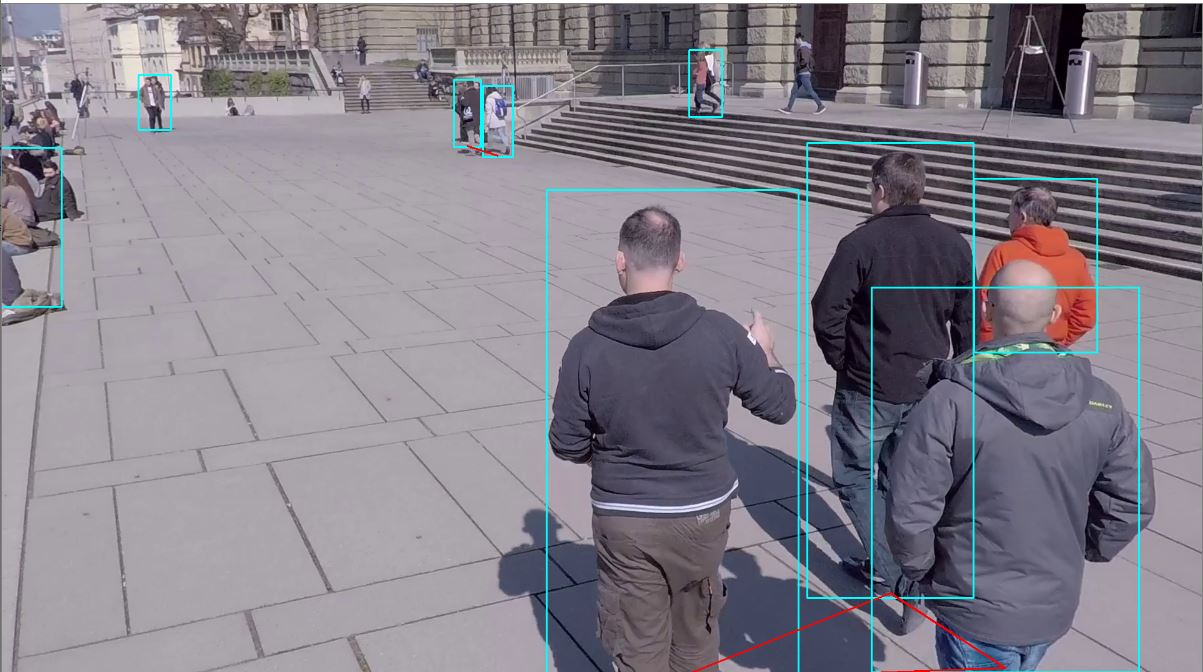
\includegraphics[width=65mm]{./images/appendix/HomographyExample1.JPG}
	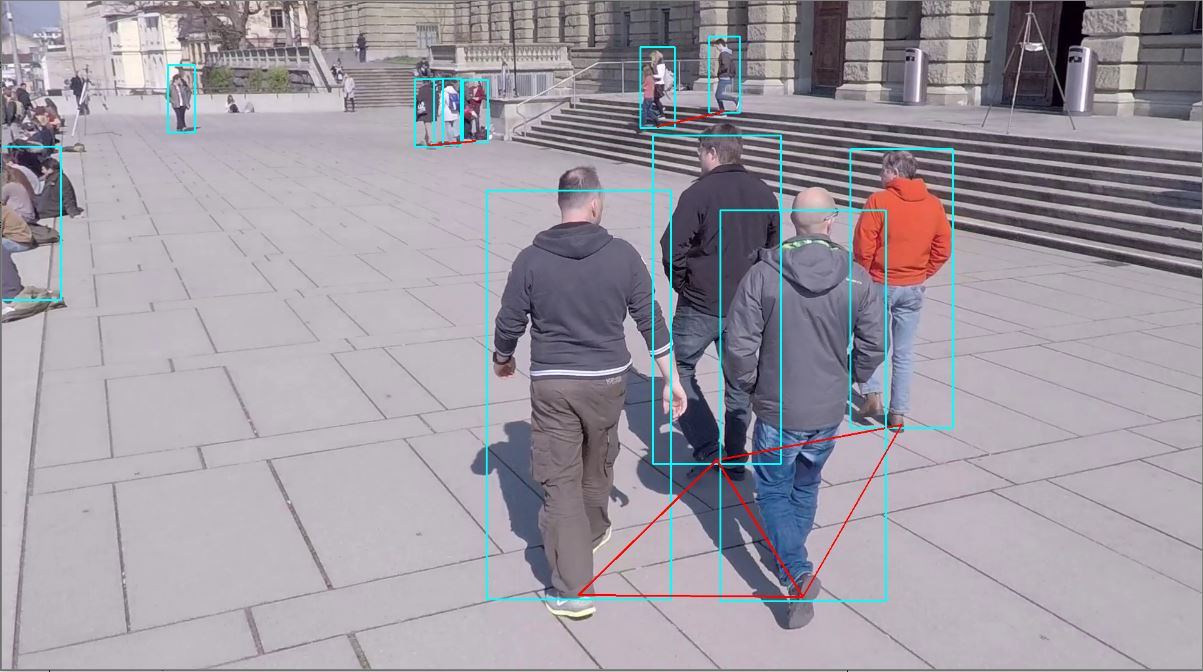
\includegraphics[width=65mm]{./images/appendix/HomographyExample2.JPG}
	
	{\footnotesize Figure 5.12: 'video 8' with homography Social Distancing detection applied.}
\end{center}

\subsection*{Estimated Homography matrix}

Another method that was tested was to use an estimated homography matrix which is formed by a OpenCV function called cv2.findHomography which takes 4 points on the image planar surface and real world surface (Kriegman D. 2007). The 4 points that correspond to the real world should create a square on the planar surface when connected, while the other 4 points which are image coordinates should correspond to where the real world coordinates are. The goal is to create a variation of the matrix acquired in the previous method to transform an image point to real world coordinates.


\vspace{2mm}

The implementation is possible due to the data that the WILDTRACK dataset provides, giving annotations of people's position in the real world within a certain frame of the video. The system can use this information for the parameters needed. While this doesn't directly use the calibrated cameras, the accuracy of the annotations were obtained by using camera calibration.

\vspace{2mm}

The outcome of the method was similar to the previous camera calibration method, but seemed less accurate overall. This is because the parameters used in 'findHomography' function did not form a proper square in the real world. Therefore, every transformed point was slightly skewed. Figure 5.13 shows how the image coordinates are transformed by the estimated homography. The group of pedestrians are still in clusters after transformation, but the perspective does not match where the people are in the real world.

\begin{center}
	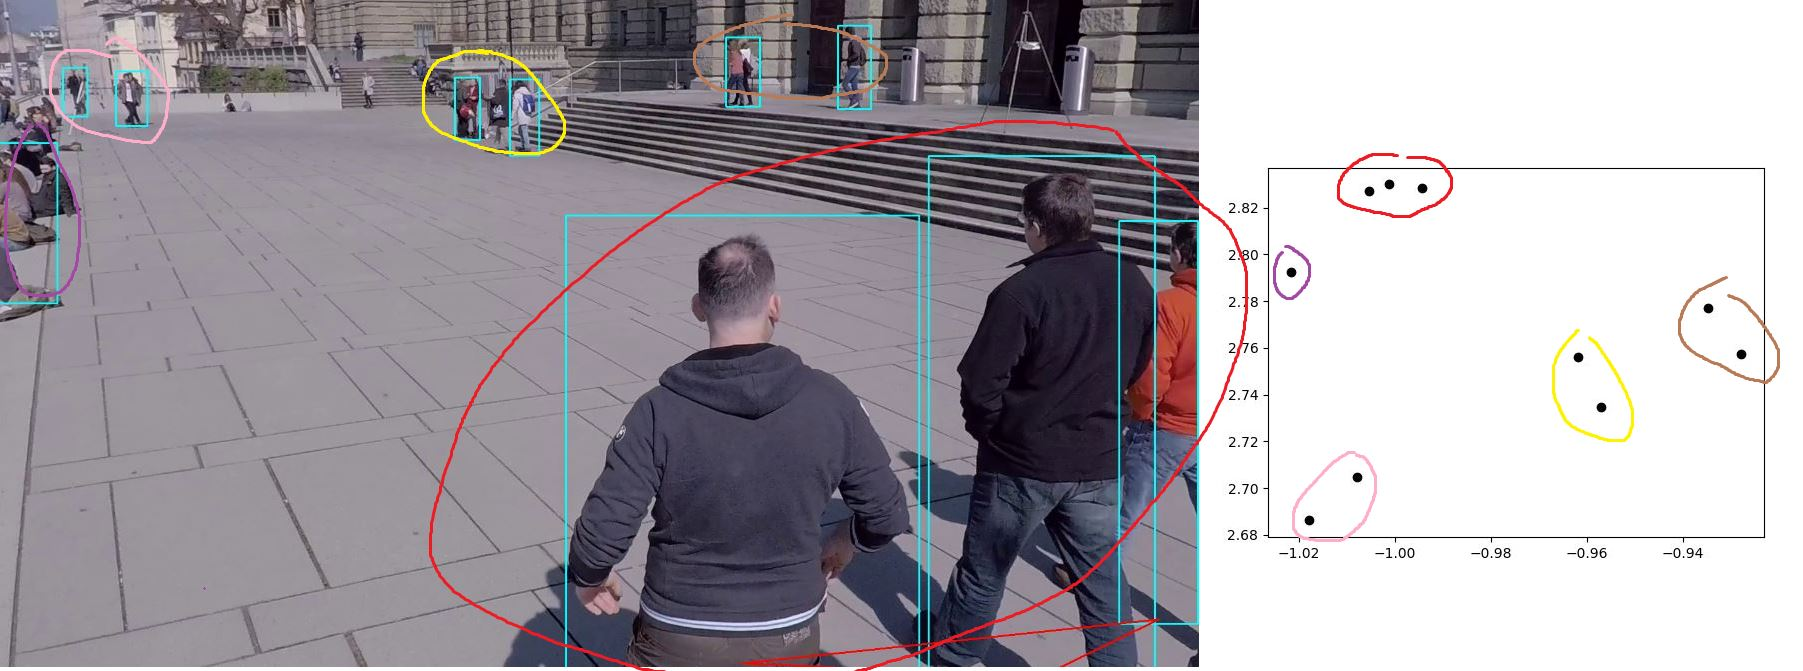
\includegraphics[width=150mm]{./images/appendix/EstimatedHomographyP.JPG}
	
	{\footnotesize Figure 5.13: 'video 8' with an estimated homography transformation plot.}
\end{center}

\subsection{Conclusion of detecting SD by camera calibration}

The camera calibration technique to form the homography matrix with both the intrinsic and extrinsic parameters is somewhat on par with accuracy of the matrix transformation for a top down view, with the added benefit of not being restricted to a quadrilateral space within the image. One of the problems with camera calibration is that the camera must be static after calibration as the extrinsic values with vary depending on the position of your camera.

\vspace{2mm}

The technique to form an estimated homography matrix from points in the real world and image plane should in theory produce very accurate results, but the parameters used in the example were inaccurate, therefore the function did not work out for this project.

\vspace{2mm}

Camera calibration can seem like a daunting task, but the only material that is needed are multiply images of a measured checker board (preferably 20 images) taken by the camera that needs calibration. (OpenCV: camera calibration, 2021)

\section{Plotting pedestrians on a top down view}

Creating a top-down view of the pedestrians will give better clarity to the beneficiaries as to where the people are in the real world. It will show how each method transforms a image point to a 3d point. Each pedestrian detected will be plotted on a black window which will be in sync with the video/image input. Like the output videos, the top-down view will draw a line between pedestrians who are close to each other. All outputs will be done with 'video 5' for easy comparisons.

\vspace{2mm}

The first and easiest method to achieve the top down view is the matrix transformation. Looking at figure 5.9, the image already has a good template to work with. The right side of the image will be replaced with a black window instead of the transformed image.

\vspace{2mm}

Figure 5.14 shows a frame of 'video 5' with the implemented top-down view over a black window. The green circles in the black window indicates people who are social distancing and yellow circles indicate otherwise. The output of the plots are well synced with the video and has a smooth transition between frames.
\begin{center}
	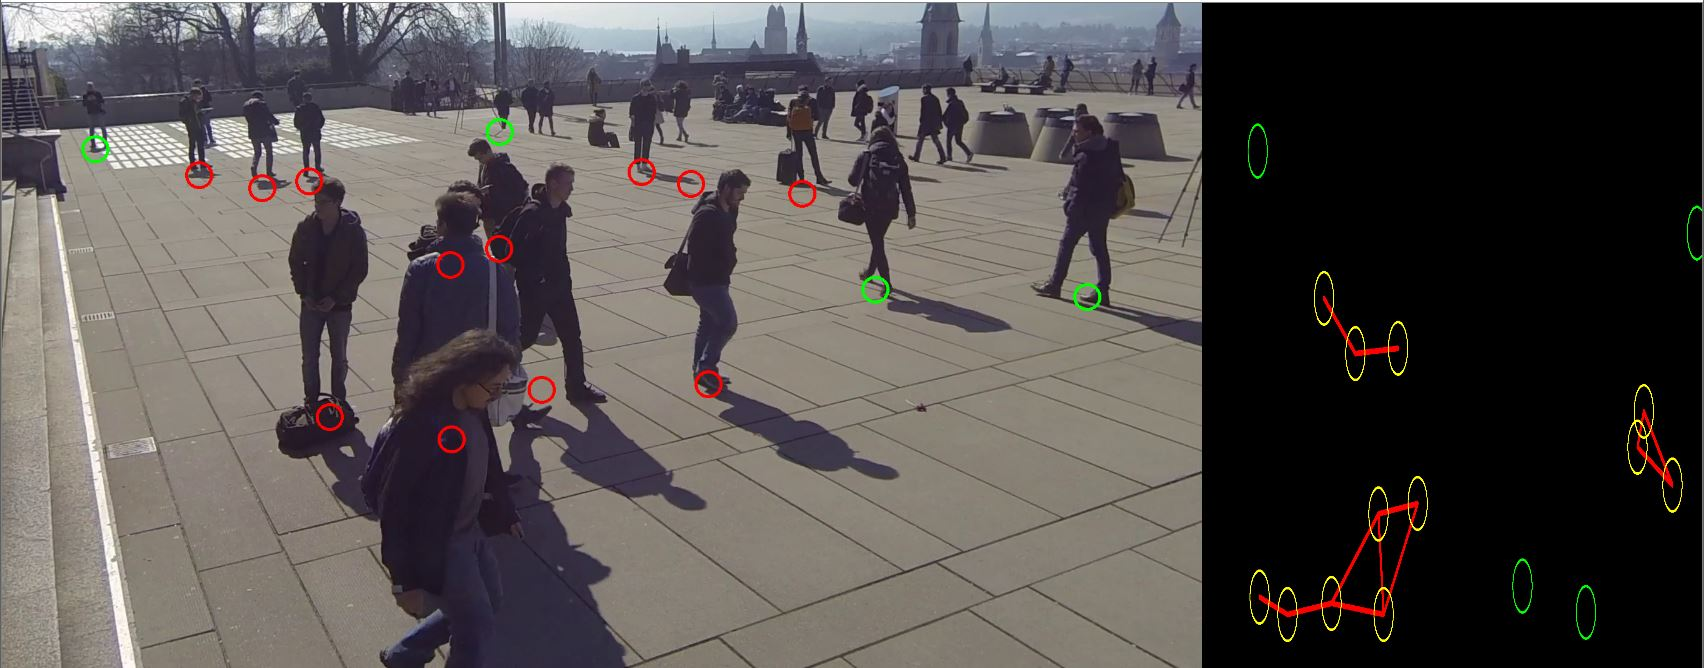
\includegraphics[width=150mm]{./images/appendix/BlackBoxMatrixTransformation.JPG}
	
	{\footnotesize Figure 5.14: 'video 5' with a top down view using matrix transformation.}
\end{center}

The next method that implemented the top-down view is the camera calibration. Unlike the matrix transformation which returned image coordinates as its output, the camera calibration has its own units where the values could be negative. Therefore plotting the points on a image plane is not sufficient enough. In order to combat this, the coordinates are normalized between 0 and 1. The normalized coordinates will then be multiplied by a number that is slightly less than the resolution of the black window to allow for every pedestrian to fit on the top-down view.

\vspace{2mm}

The first iteration did successfully plot all of the identified pedestrians on the image plane, but a problem occurs when the each frame is treated independently from one another. The normalization works by making the largest coordinate value after transformation the upper bound of the normalization (This is equal to one.) and the smallest coordinate value to be the lower bound (This is equal to zero). Since the upper and lower bound changes every frames, the coordinates are not stable when plotted on the black screen and creates chaos. Appendix 9a shows how two different frames that are close in time plot each pedestrian with different lower and upper bounds.

\vspace{2mm}

The solution to solving this problem is snapshotting the upper and lower bounds of the first frame of the video and passing the parameters to the next consecutive frame to create a global normalization across all frames of the video. The upper and lower bounds will be updated if the current bounds are a better fit. The plots are now more stable and less chaotic when moving onto the next frame. Figure 5.15 shows the final output of creating a top down view using the camera calibration output coordinates.

\begin{center}
	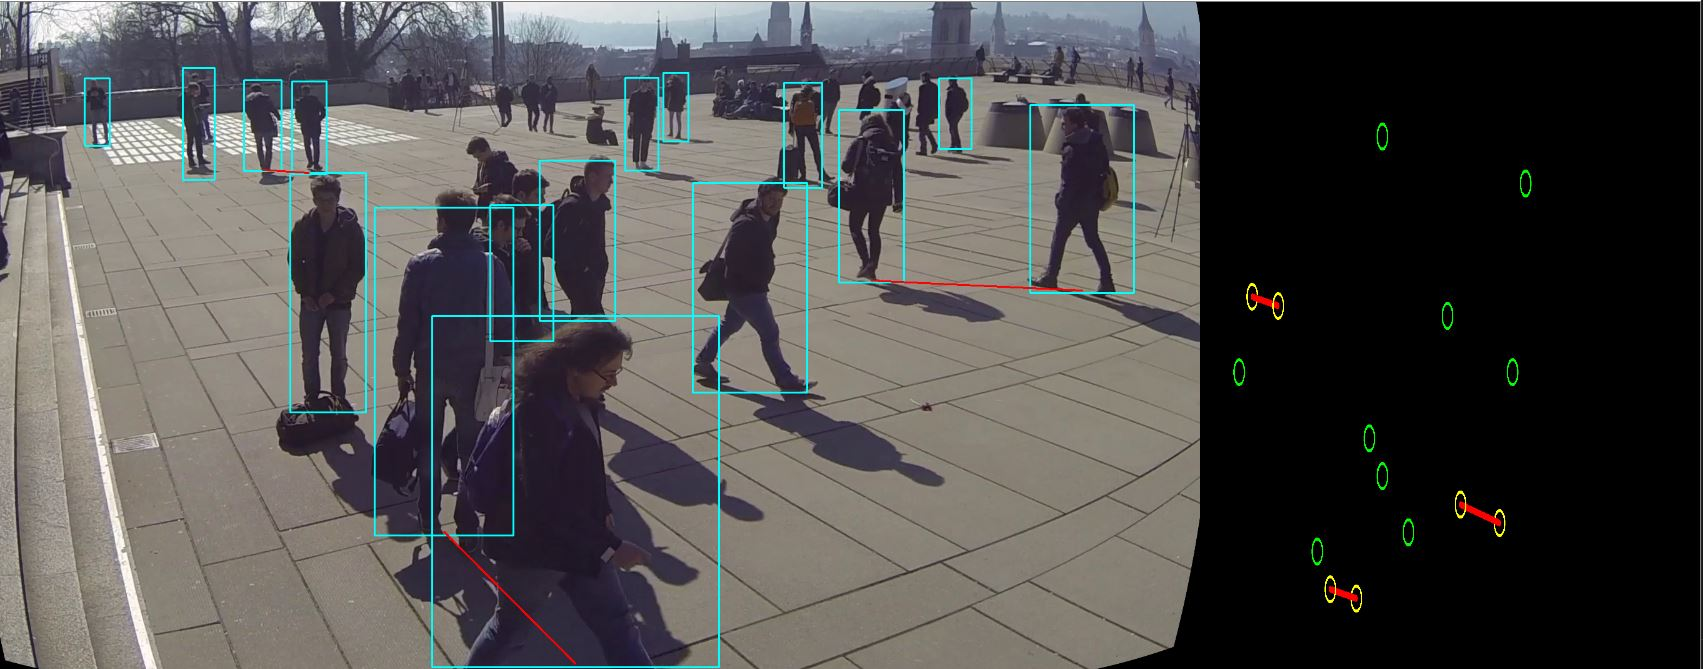
\includegraphics[width=150mm]{./images/appendix/Stable.JPG}
	
	{\footnotesize Figure 5.15: A frame of 'video 5' with the final top down view output of camera calibration.}
\end{center}

\subsection{Conclusion of creating a top down view.}

This section discusses creating a top-down view using two out of the three methods used in the report. While the other method (SD by bounding box) is possible, the results are probably not as accurate as the others, therefore producing an output seemed redundant.

\vspace{2mm}

When comparing the two methods discussed, the camera calibration is more flexible with pedestrian plotting and is not limited to a quadrilateral space in the image plane. But looking at figure 5.15, the angle of the black window output can seem confusing to the user. There are solutions to the problem such as applying a rotation matrix to the coordinates, but overall both methods are very successful at what task was trying to achieve.

\section{Identifying groups of people and marking them as ’safe’}

Currently the system mainly benefits beneficiaries who work in small offices as every individual is marked independently to one another. If the system were to be used in a more public area, the system would need to be able to identify people in groups as there could be a group of both a parent and child. Having a pair detected as not 'social distancing' could do more harm than good.

\vspace{2mm}

The first problem that the system must tackle is that we can not locate the same person from one frame to another. Not having this information means we can not pair pedestrians together. A solution to solving this problem is to create a map that allocates a key to pedestrian with information that hold the current image coordinates of the person. This map is passed onto the next frame, where the items in the map will be compared to the pedestrians detected in the current frame. Since people move from frame to frame, the system detects pairs who have move under x amount of pixels away from their previous frame using boundaries. Since the object detection does not return a list of people detected in the same order as the previous frame, we will need to use a  O($n^2$) loop to compare.
\vspace{2mm}

Figure 5.16 demonstrates the algorithm with 2 frames from the same video that are seconds apart. Most pedestrians are able to maintain their key, but due to the limitations of the object detection discussed in section 5.1.3, the 'yolov3' architecture may fail to identify a person within a single frame, therefore a new key is given to the pedestrian (A new key '10' was generated for the person who had key '2' in the left image).

\begin{center}
	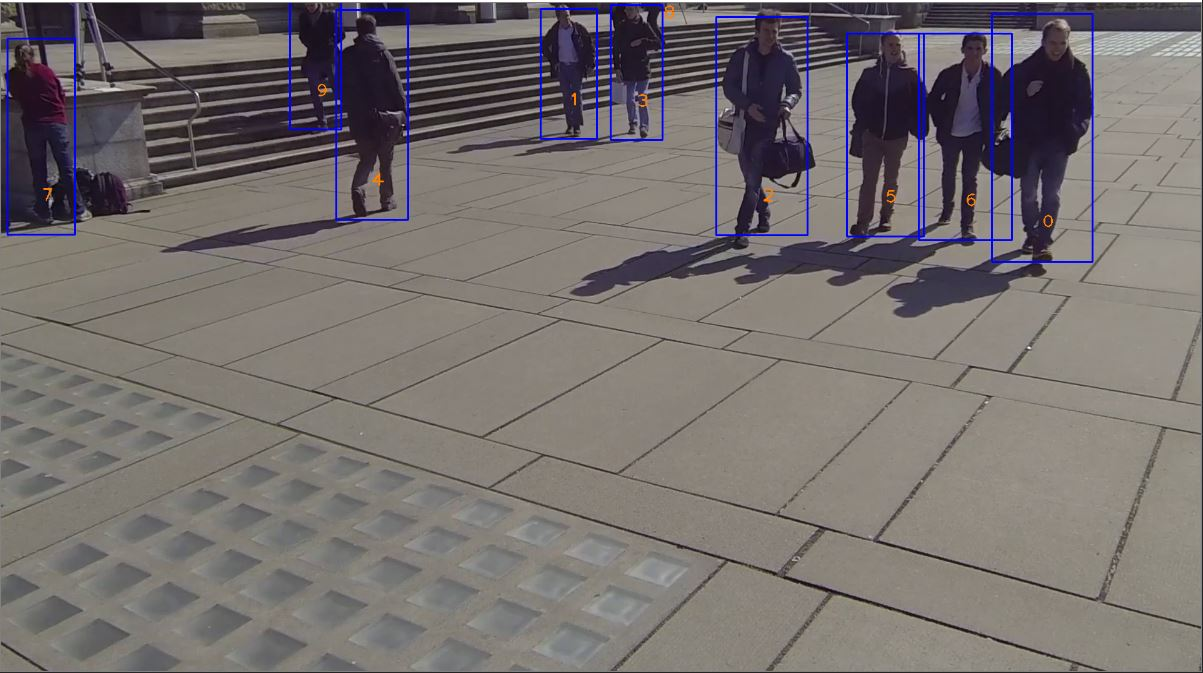
\includegraphics[width=65mm]{./images/appendix/Key1.JPG}
	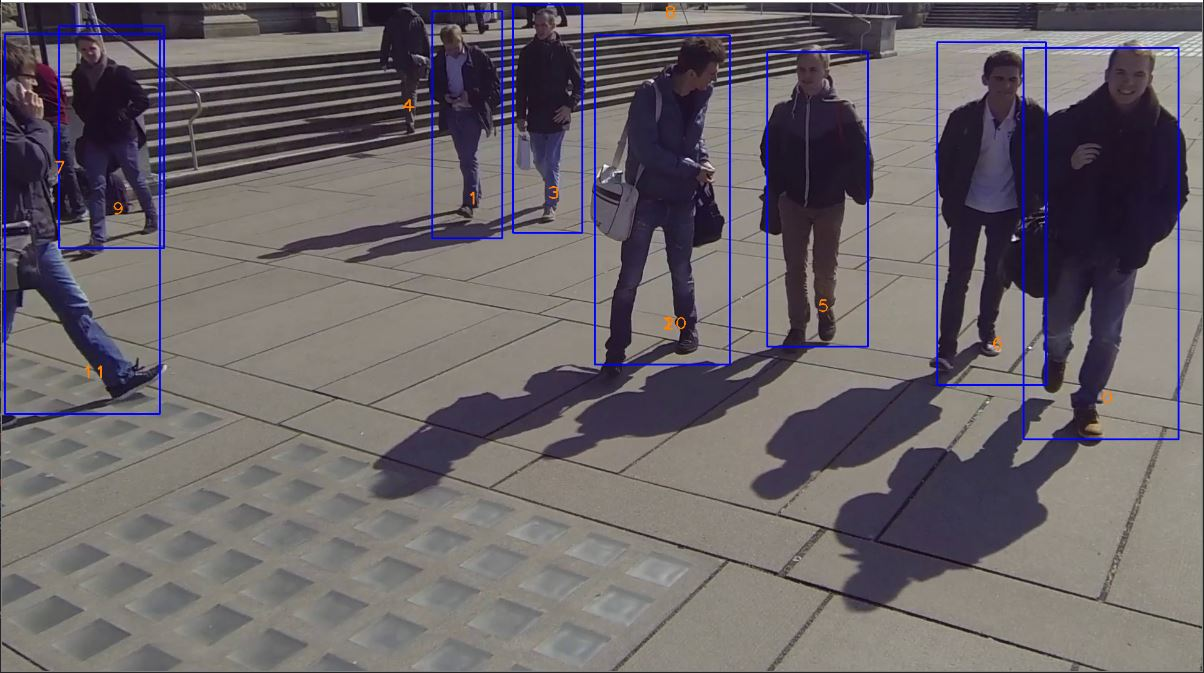
\includegraphics[width=65mm]{./images/appendix/Key2.JPG}
	
	{\footnotesize Figure 5.16: 'Video4' with keys given to pedestrians.}
\end{center}

Now that the system can keep track of individual pedestrians, the system will need to keep track of people who are not 'social distancing' together. The homography function returns a list of paired people who are close to each other (not 'social distancing'). Figure 5.17 shows the list that the homography function returns on the left, while the list on the right is the outcome of linking each pair in a single list. 

\begin{center}
	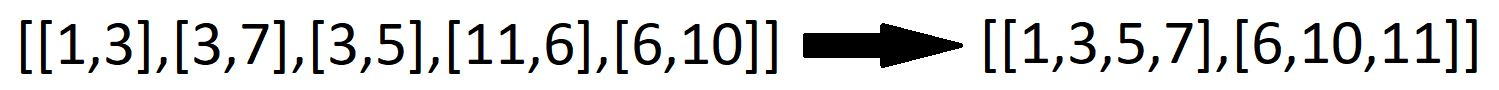
\includegraphics[width=150mm]{./images/appendix/Linked.JPG}
	
	{\footnotesize Figure 5.17: pairs of numbers linked together in a single list}
\end{center}

The system was able to achieve the list on the right from the list on the left in figure 5.17 using multiple for loops (Time complexity O(n$^2$)). Figure 5.18 highlights the group of people who were not 'social distancing' on the first frame of 'video 7' (Key of [1,2,5]) with a green border. Later on in the video (right image), the pedestrian with key number 5 was not detected by the model for 1 frame, therefore the pedestrian got a new key of 37 is not longer highlighted to be part of the group.

\begin{center}
	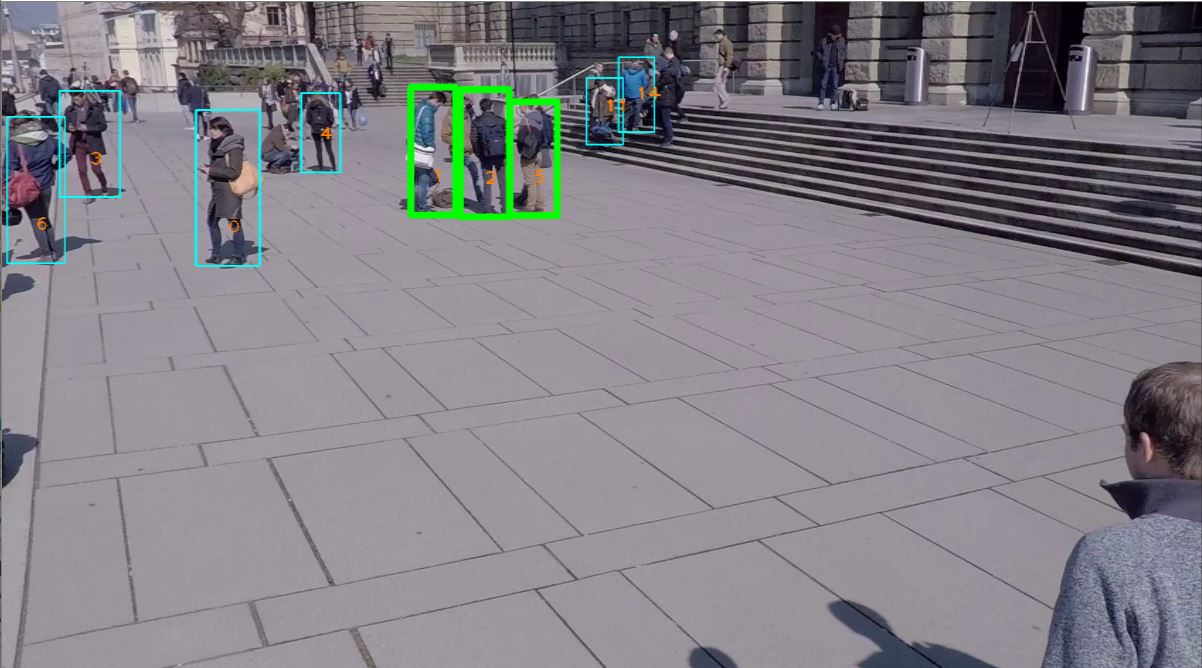
\includegraphics[width=65mm]{./images/appendix/Groups1.JPG}
	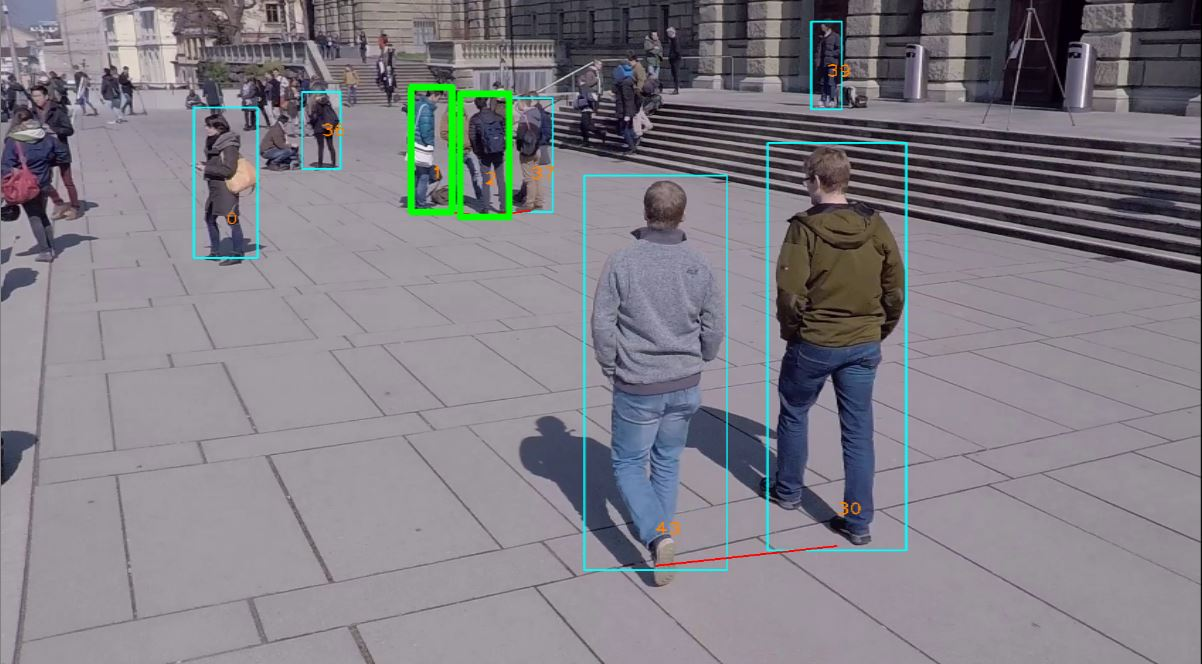
\includegraphics[width=65mm]{./images/appendix/Groups2.JPG}
	
	{\footnotesize Figure 5.18: 'Video 7' with groups of people highlighted.}
\end{center}

To allow new people to be grouped, the system will group any pedestrians who are within the red zone in figure 5.19. The group must not be 'social distancing' in the red area to be eligible for grouping. The red area acts as a zone that identifies people as entering the camera view. While there is a possibility that people can be identified as groups when leaving the camera frame, they will only be seen as a group for only a few seconds.

\begin{center}
	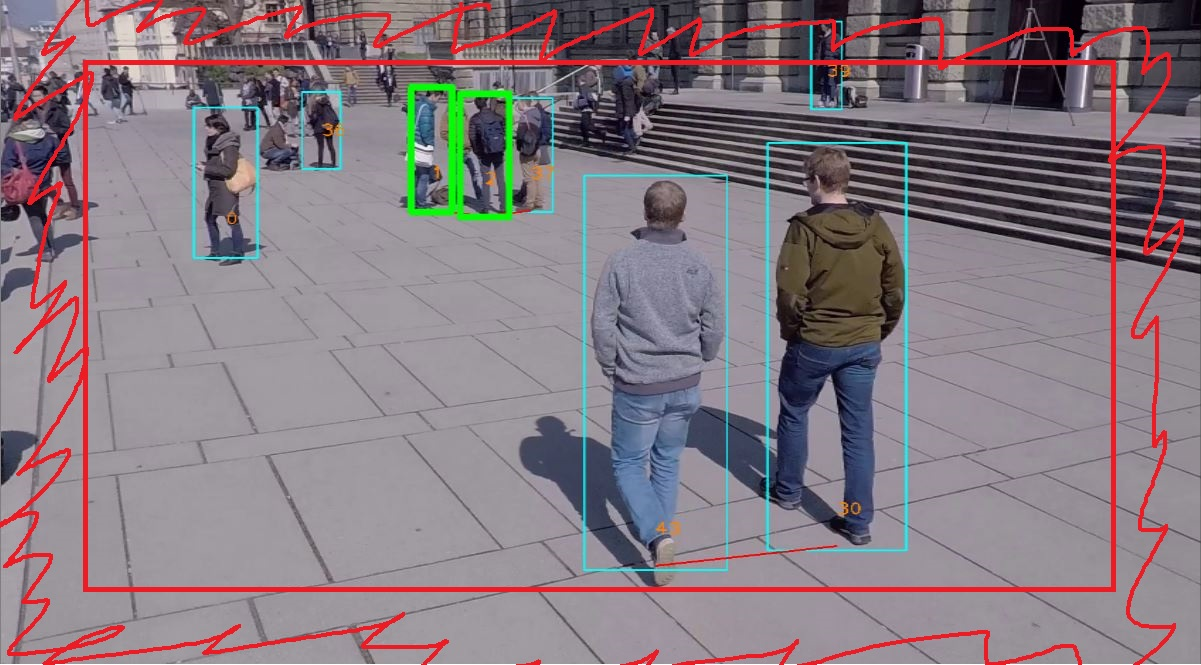
\includegraphics[width=65mm]{./images/appendix/GroupZone.JPG}
	
	{\footnotesize Figure 5.19: 'Video 7' highlighting the 'group' zone.}
\end{center}

Figure 5.20 shows that the group implementation is successful. The system is able to identify groups of people who are coming into the camera frame and marking them with a green border. But due to the limitations of the 'yolov3' architecture, it is difficult to maintain the same key on the same person, therefore the pair coming into frame loses their green border over time.  

\begin{center}
	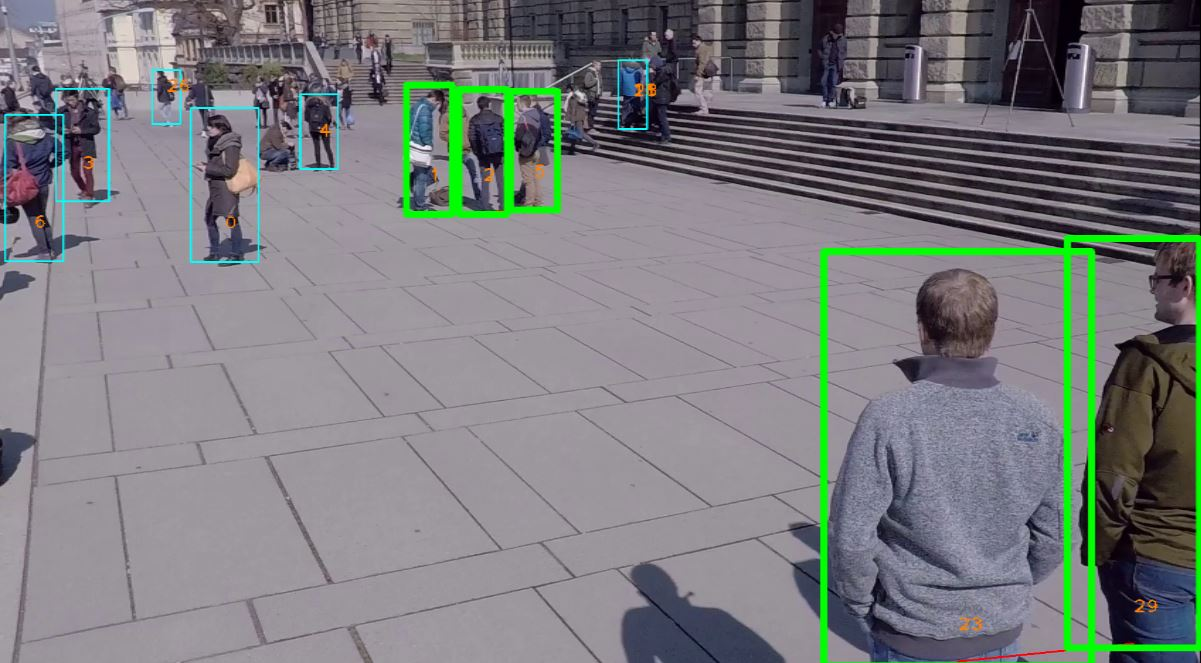
\includegraphics[width=65mm]{./images/appendix/AddingGroups.JPG}
	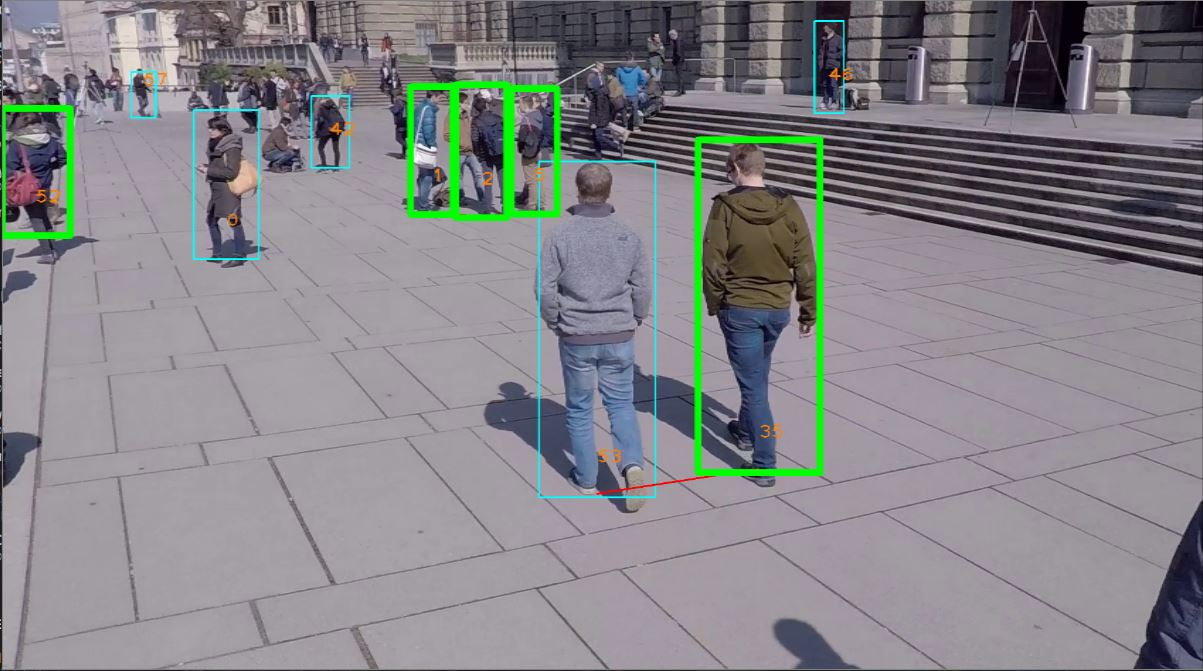
\includegraphics[width=65mm]{./images/appendix/AddingGroups2.JPG}
	
	{\footnotesize Figure 5.20: 'Video 7' with 'group' zone implemented.}
\end{center}

\subsection{Conclusion of identifying groups of people and marking them as 'safe'.}

The goal of identifying groups of people did work very well, but the current code relies too heavily on how well the object detector performs. It must keep track of each person at all times, but this is beyond the technology of 'yolov3'. The code also makes too many assumptions on the pedestrians movement, the person must keep moving with their group side by side. The assumption falls flat when there is a stationary person within the 'group' zone (Figure 5.20).

\vspace{2mm}

The algorithm used exerts a lot of computational power, using multiple 'for' loops that are time complexity O(n$^2$) and O(n$^3$) to calculate groups of people for only a single frame. When lowering the confidence of the 'yolov3' model to introduce more bounding boxes, the hardware is unable to handle the amount of calculations done.

\vspace{2mm}

The final algorithm is too volatile to be used in a commercial setting and doesn't work well in crowded areas due to the chaos and limitations of the object detector. The current iteration of 'group' detection is not suited for identifying groups of people who have parents and children due to the lack of consistency.

\chapter{Discussion and conclusion}

\section{Discussion}

\subsection{Project impact}

The title of the report "Social distancing detection with computer vision techniques" was fully met by using a pre-trained deep learning model to detect pedestrians within an image which is then used to calculate 'social distancing' with various different methods. The report demonstrates multiple ways beneficiaries can tackle the problem of keeping a safe distance from each other by monitoring their own movement with the system.

\vspace{2mm}

The result section features a similar solution to the existing system in the literature review which is matrix transformation. The added feature that this report introduces was the use of camera calibration and distortion coefficients to acquire more accurate results. The report also discussed two other approaches on top of the matrix transformation.

\subsection{Project achievements and flaws}

The camera parameters found in the WILDTRACK dataset is not specifically suited for the matrix equation in section 5.5 because of the use of multiple cameras, therefore the results seen in section 5.5 are not as accurate as they could be. This is an oversight by the author, and could have been avoided if researching about camera parameters, equations, and other datasets was done prior to starting the project. Overall, the results seen in section 5.5 still achieves the goal of calculating social distancing with a good accuracy. 

\vspace{2mm}

While the focus of the report is social distancing, the results discusses a method that is created by the author of identifying groups of people while keeping track of who's who from one frame to the next. This implementation is very successful and can potentially be applied to other problems such as tracking a car within traffic or used for surveillance purposes.

\vspace{2mm}

While the algorithm for marking groups of pedestrians as 'safe' seen in the report is complex, the movement of pedestrians is too chaotic to produce a perfect outcome. The algorithm has a clear downside of being too computational heavy and too reliant on the object detector and assumptions about pedestrian movement, the algorithm would work better with perfect conditions but this is beyond the capabilities of the current computer vision technology. 

\vspace{2mm}

The section of analysis the 'yolov3' architecture is very important for the project and beneficiaries. The analysis presents a good understanding of the limitation of the deep learning model and how it can effect the overall outcome of the project. And it also provides information about how different camera qualities perform and how the user must tune the parameters in order to detect social distancing. The conclusion of the results seen in section 5.1 is that the system does work with lower quality cameras but if not tuned properly, too much information is lost.


\subsection{Project management and improvements}

Every development phase has resulted in a satisfactory or complete solution. Each phase/sprint was achieved within the time frame given without needing to compensate for more time. Research for each phase was done a day before the sprint started to ensure completion of code and time to test. The writing of the report however proved difficult in some areas for the author due to lack of experience.

\vspace{2mm}

An improvement that could be made for this project is to use a more suited dataset for the camera parameter equations. Doing such will produce higher accuracy results.

\vspace{2mm}


\section{Conclusion}

The report is able to showcase three different methods to detecting social distancing, The author gained knowledge on camera calibration and how different matrix transformations can solve perception within an image. The author also produced their own method to tackling perception by adding linear scalars to the pixels of the images, as-well-as developing a method to detecting groups of people. 

\chapter*{References}
\begin{verbatim}

Chavdarov, T., Baqué, P., Bouquet, S., Maksai, A., Jose, C., Lettry,
 L., Fua, P., Van Gool, L. and Fleuret, F., 2017.
The wildtrack multi-camera person dataset 
p.3., p.5., p.7. 

Coifman, B., Beymer, D., McLauchlan, P., Malik, J. (1998).
A real-time computer vision system for vehicle tracking and traffic 
surveillance. Transportation Research Part C: Emerging Technologies

Doc.opencv.org. 2021. OpenCV: Camera Calibration [online Available at:
https://opencv-python-tutroals.readthedocs.io/en/latest/py_tutorials/
py_calib3d/py_calibration/py_calibration.html/ 
[Accessed 01/04/2021]}

Docs.opencv.org. 2021. Camera Calibration and 3D Reconstruction — 
OpenCV 2.4.13.7 documentation. [online] Available at:
<https://docs.opencv.org/2.4/modules/calib3d/doc/
camera_calibration_and_3d_reconstruction.html>
[Accessed 13 March 2021].

Docs.opencv.org. 2021. OpenCV: Basic concepts of the homography 
explained with code. 
[online] Available at: 
https://docs.opencv.org/master/d9/dab/tutorial_homography.html
[Accessed 15 March 2021].

Hochreiter, Sepp and Jurgen Schmidhuber. 1997. 
"Long Short-Term Memory. Neural Computation" 
:1735–1780.

Kriegman D. URL https://cseweb.ucsd.edu/classes/wi07/cse252a/
homography_estimation/homography_estimation.pdf 
[Accessed 21 February 2021].



Lewis, K. and Kuhfeld, M., 2021. 
How is COVID-19 affecting student learning?. [online] 
Brookings. Available at: <https://www.brookings.edu/blog/
brown-center-chalkboard/2020/12/03/
how-is-covid-19-affecting-student-learning/> [Accessed 7 April 2021].

Lin, T., Maire, M., Belongie, S., Bourdev, L., Girshick, R., 
Hays, J., Perona, P., Ramanan, D., Zitnick, C. and Dollar, P., 2021.
Microsoft COCO: Common Objects in Context. [online] Arxiv.org.
 Available at:
<https://arxiv.org/pdf/1405.0312.pdf> [Accessed 11 February 2021].

López-Cifuentes A.,Escudero-Viñolo M., 2018. 
Semantic Driven Multi-Camera Pedestrian Detection

Metaxas, D., 1997. Physics-Based Deformable Models. Boston, MA: Springer US
, p.9.

REDMON J., FARHADI A. "YOLOv3: An Incremental Improvement"

Redmon, J., 2021. YOLO: Real-Time Object Detection. 
[online] Pjreddie.com. 
Available at:
<https://pjreddie.com/darknet/yolo/> [Accessed 11 February 2021].

Remondino, Fabio, Fraser, Clive. (2005). 
Digital camera calibration methods: Considerations and comparisons 36. 

Robert Collins (date?) URL 
http://www.cse.psu.edu/~rtc12/CSE486/lecture16.pdf 
[Online; accessed 20/03.2021]

SZELISKI, R., 2020. COMPUTER VISION. SPRINGER NATURE, p.5.

"Wikipedia. Pinhole camera model — wikipedia, the free encyclopedia, 2017b. 
URL
https://en.wikipedia.org/w/index.php?title=Pinhole_camera_model&oldid=782167557. 
[Online; accessed 20/03.2021].

Y. C. Hou, M. Z. Baharuddin, S. Yussof and S. Dzulkifly, 
"Social Distancing Detection with Deep Learning Model," 2020

\end{verbatim}

\chapter*{Appendix}

\section*{Appendix 1: PDD}

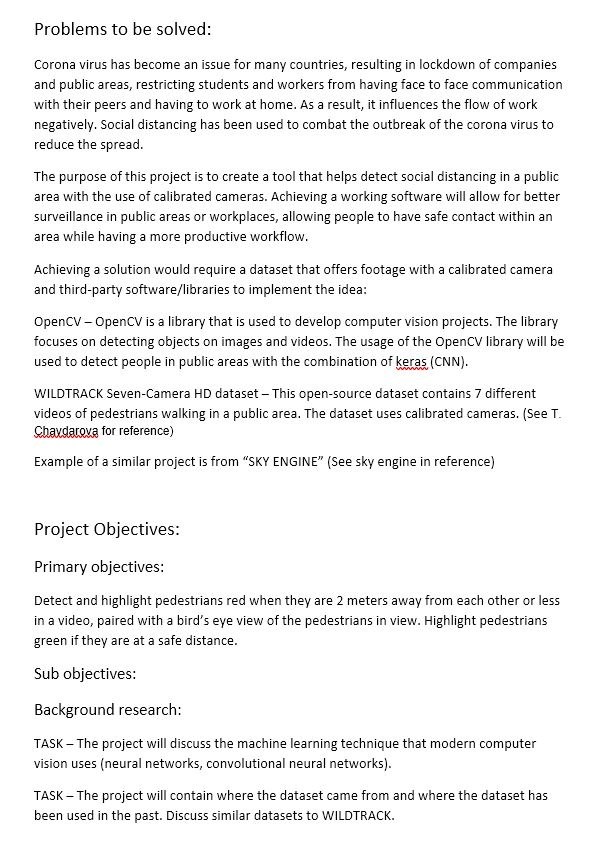
\includegraphics[width=130mm]{./images/appendix/PDD1.JPG}

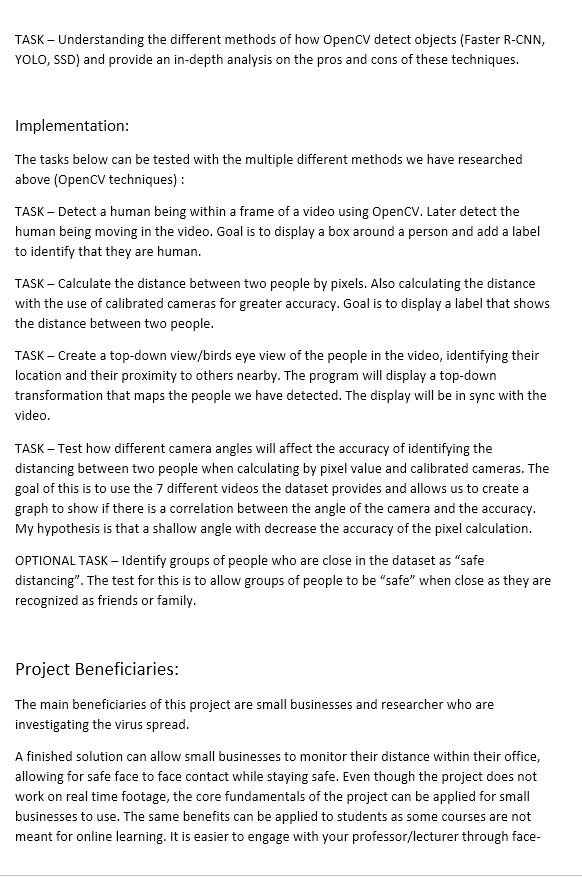
\includegraphics[width=160mm]{./images/appendix/PDD2.JPG}

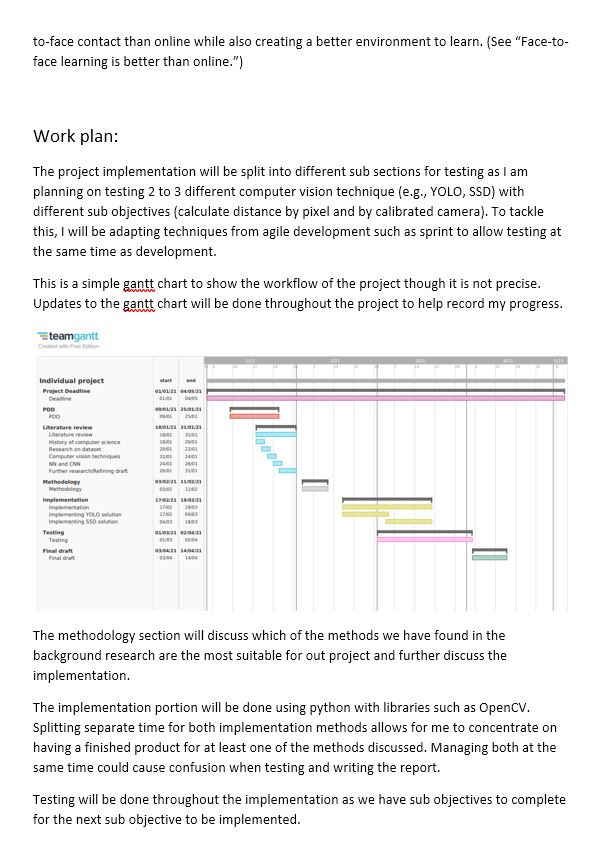
\includegraphics[width=160mm]{./images/appendix/PDD3.JPG}

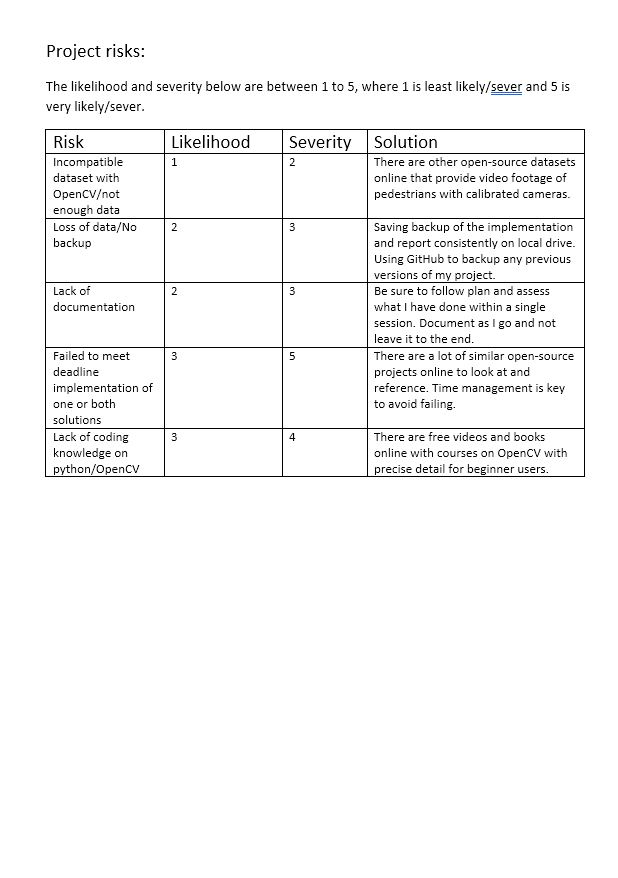
\includegraphics[width=160mm]{./images/appendix/PDD4.JPG}

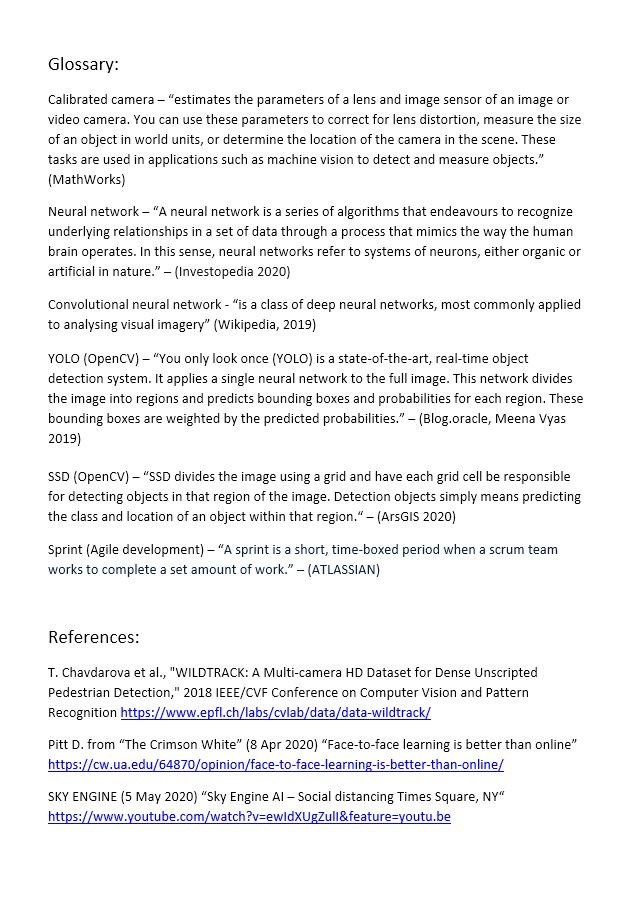
\includegraphics[width=160mm]{./images/appendix/PDD5.JPG}

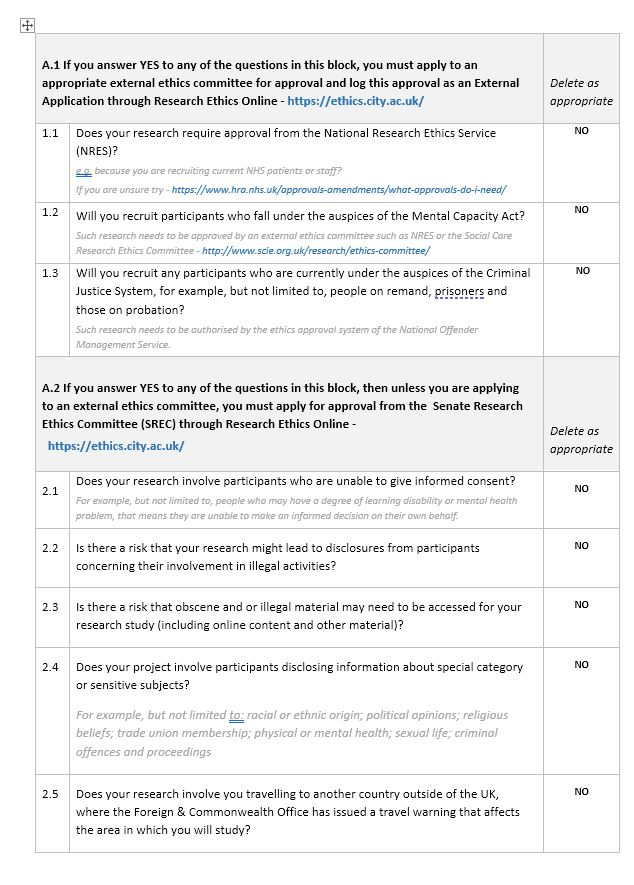
\includegraphics[width=160mm]{./images/appendix/PDD6.JPG}

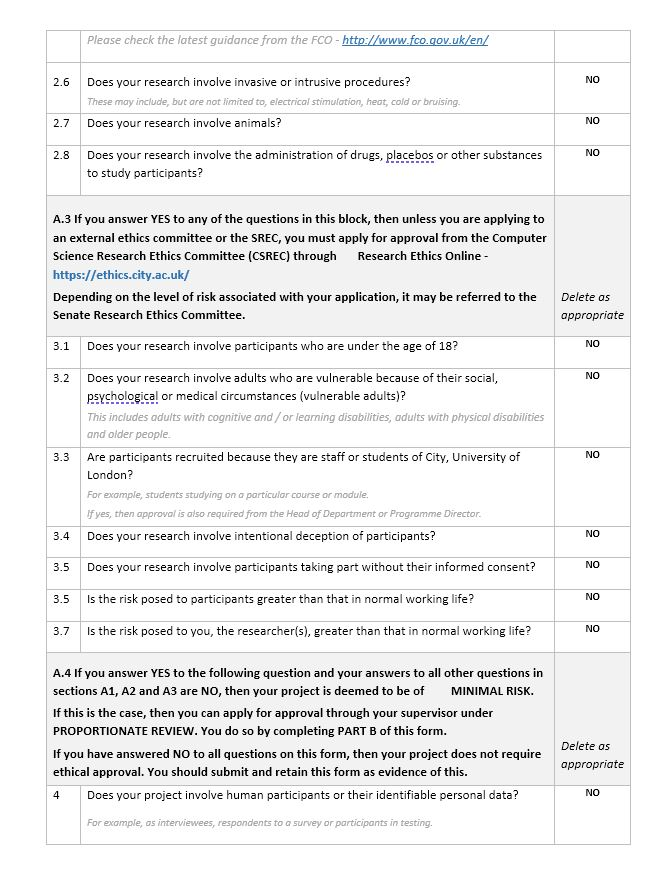
\includegraphics[width=160mm]{./images/appendix/PDD7.JPG}

\section*{Appendix 2: YOLO flowchart}

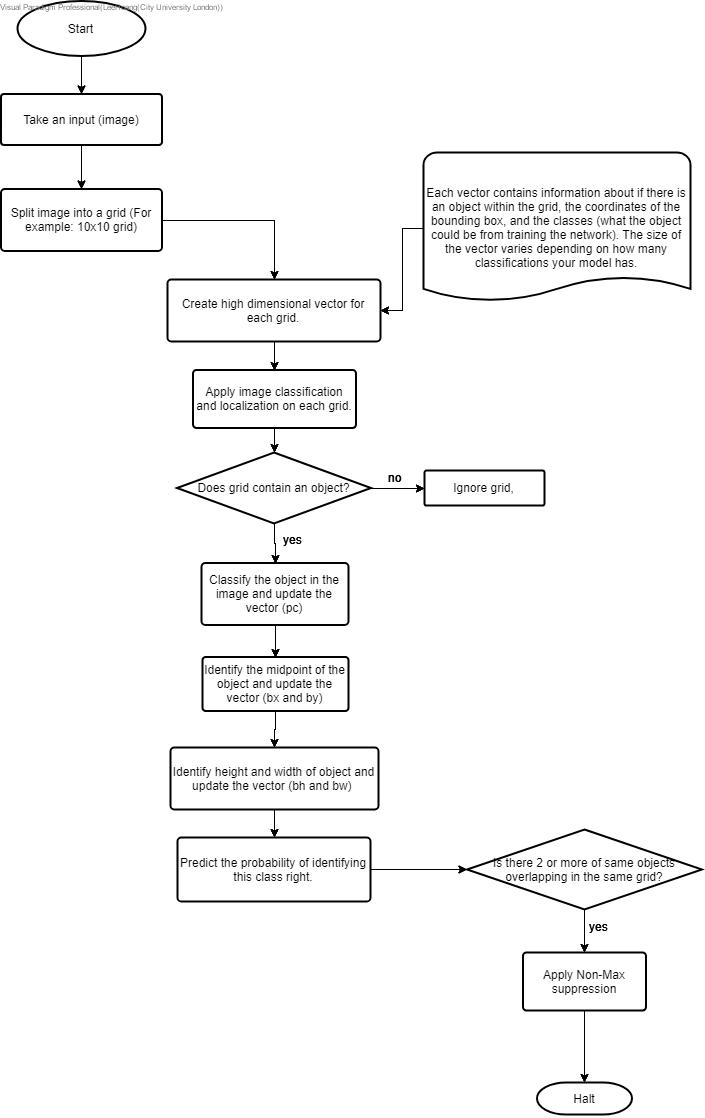
\includegraphics[width=110mm]{./images/YOLO.jpg}

\pagebreak
\section*{Appendix 3: System class diagram}

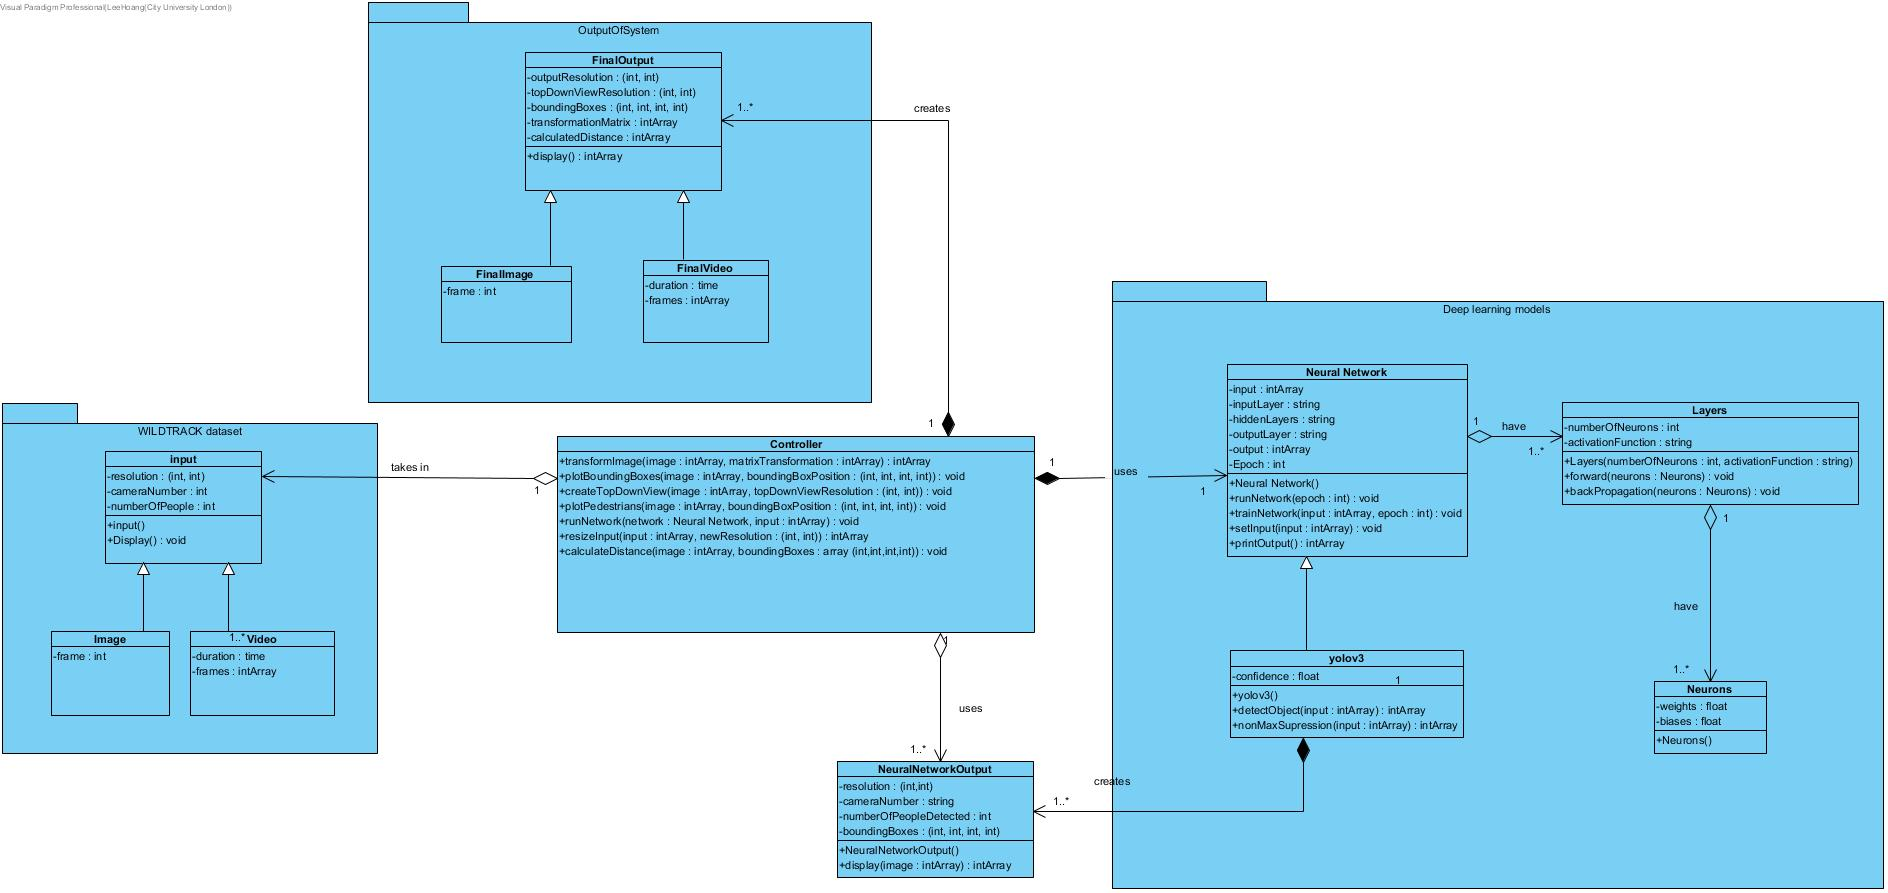
\includegraphics[angle = 90,width=100mm]{./images/SD Class diagram.jpg}

\pagebreak
\section*{Appendix 4: 5.1 outputs}

a)

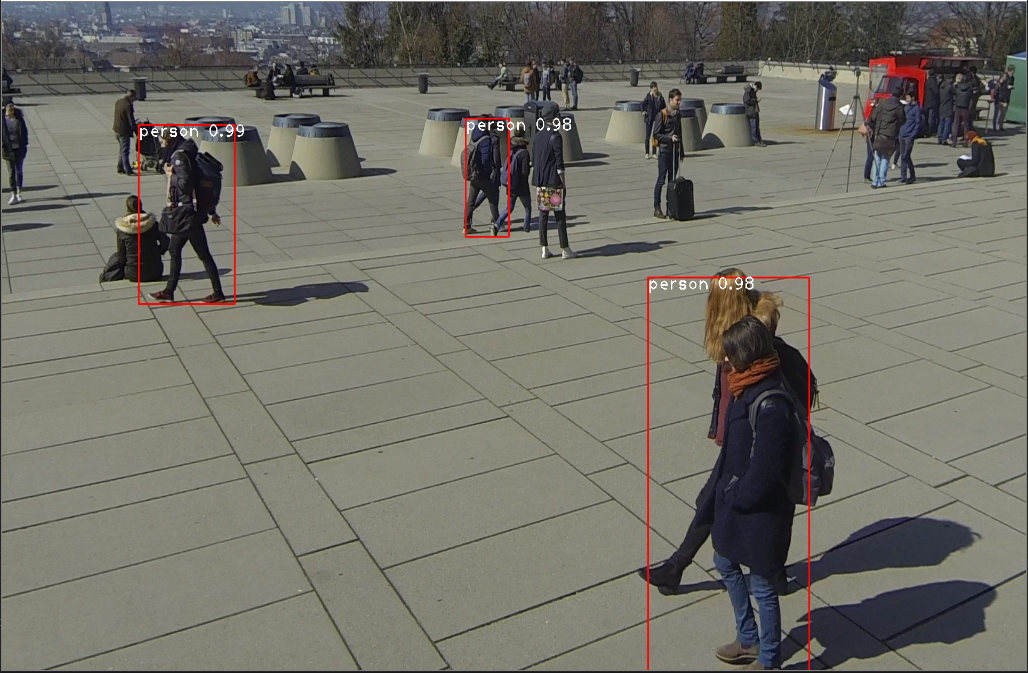
\includegraphics[width=120mm]{./images/appendix/image298confidence.PNG}

b)

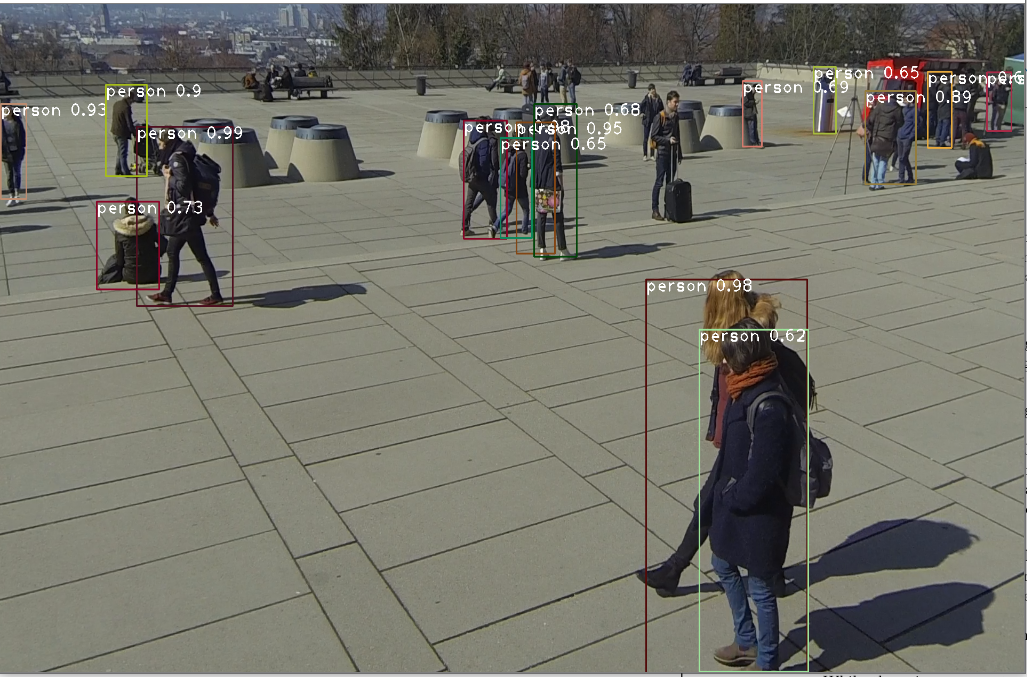
\includegraphics[width=120mm]{./images/appendix/NMS0.6.PNG}

c)

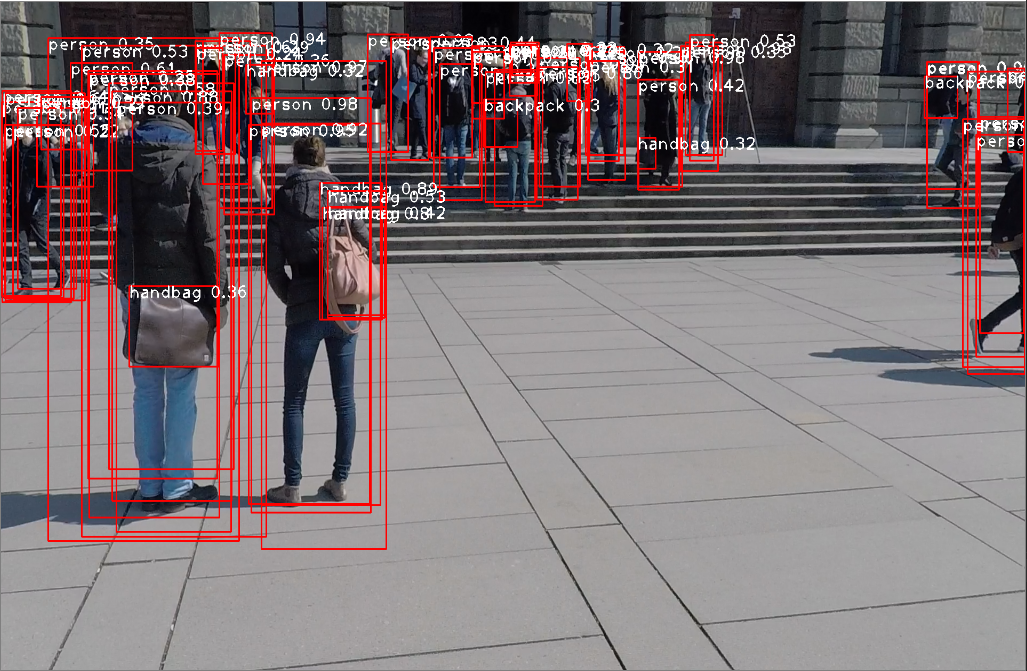
\includegraphics[width=70mm]{./images/appendix/NoConfidenceNoAug.PNG}
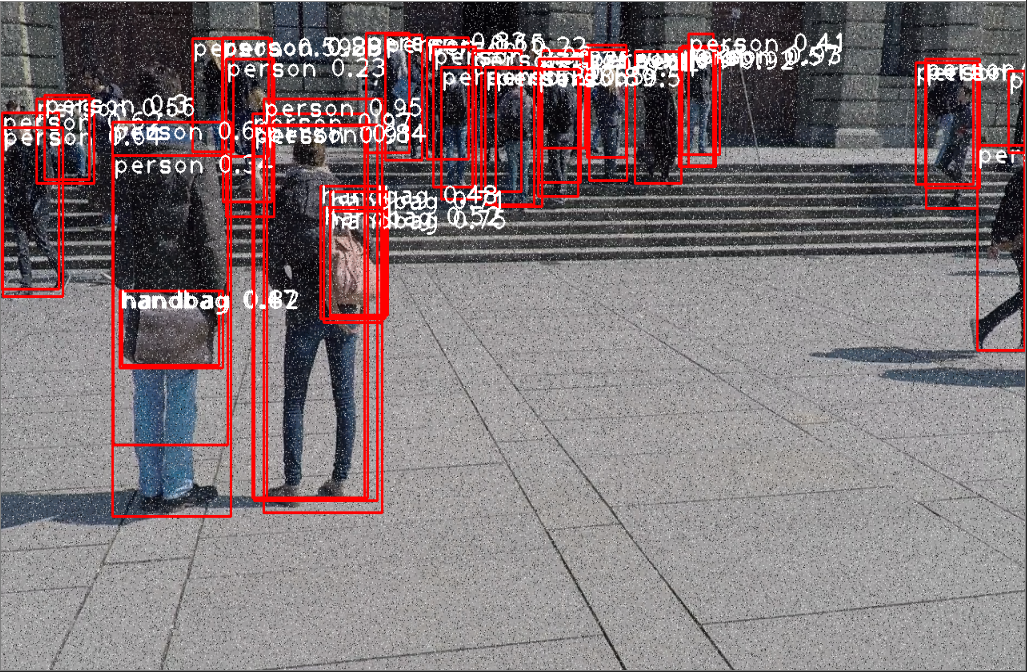
\includegraphics[width=70mm]{./images/appendix/NoConfidenceAug10.PNG}

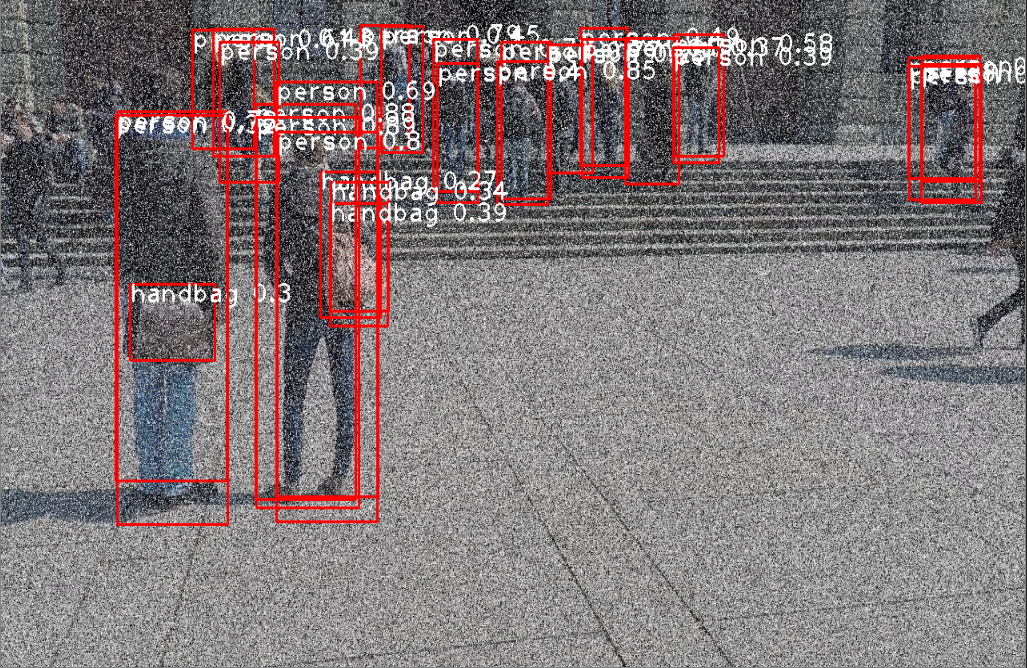
\includegraphics[width=70mm]{./images/appendix/NoConfidenceAug40.PNG}
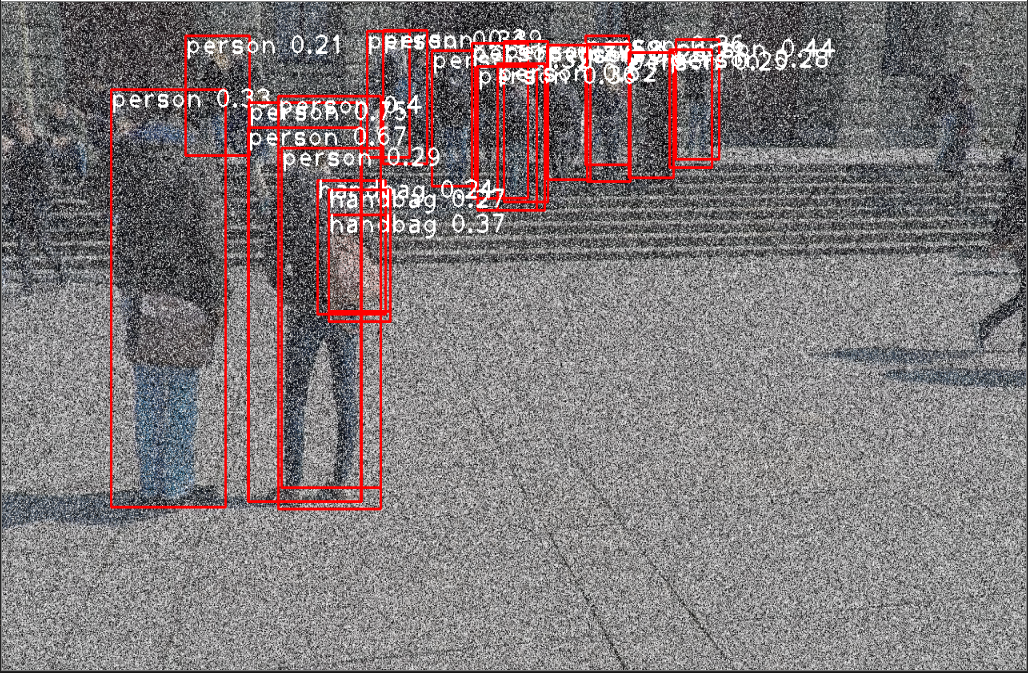
\includegraphics[width=70mm]{./images/appendix/NoConfidenceAug50.PNG}

\pagebreak
\section*{Appendix 5: 5.2 outputs}

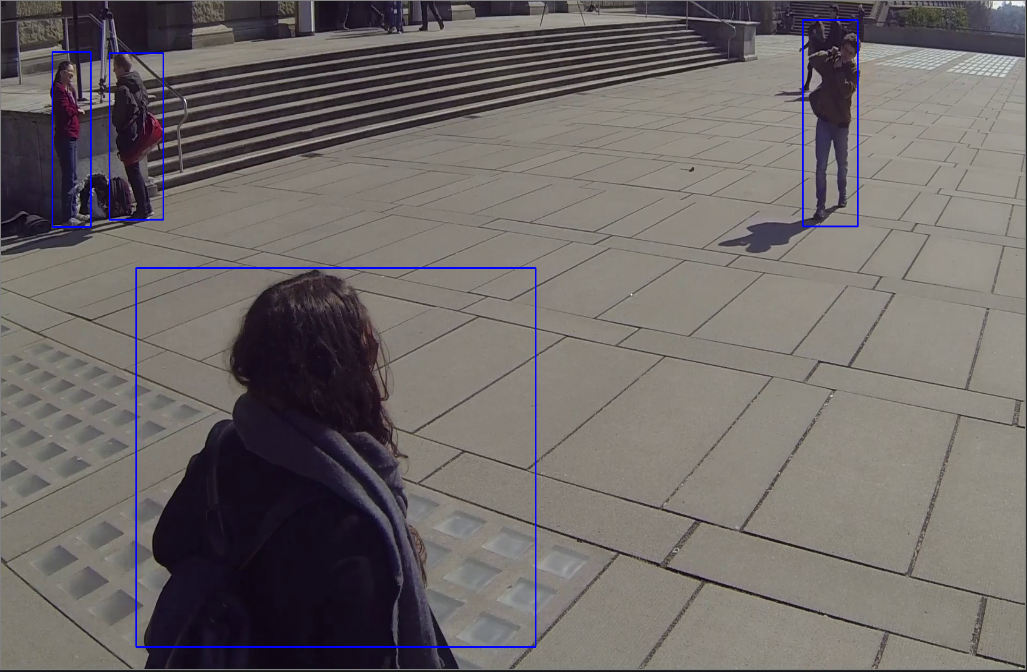
\includegraphics[width=70mm]{./images/appendix/Video3output1.PNG}
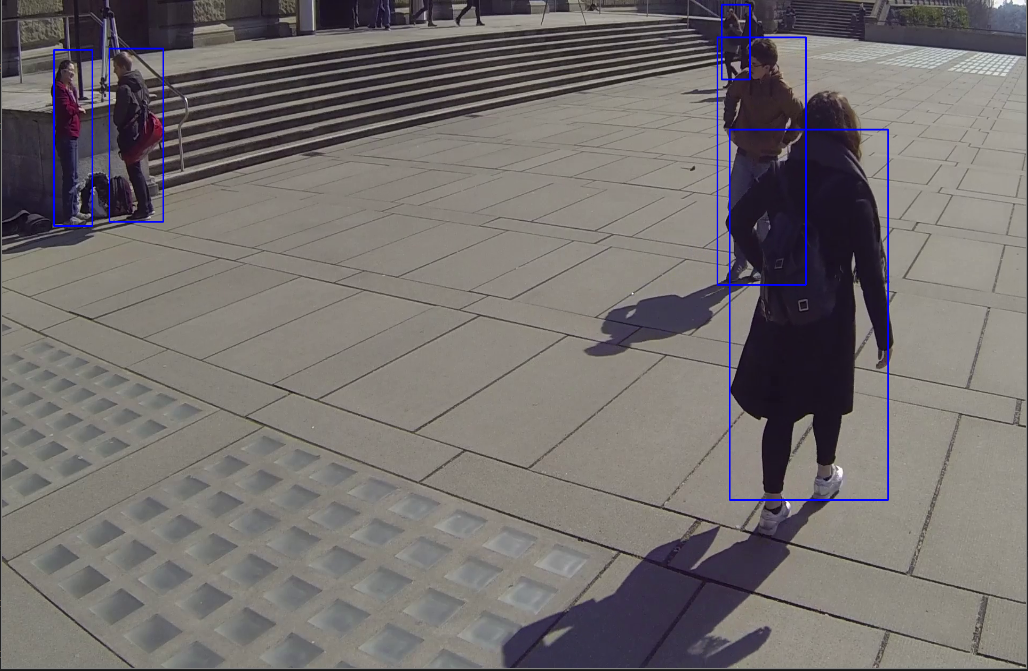
\includegraphics[width=70mm]{./images/appendix/Video3output2.PNG}


\includegraphics[width=70mm]{./images/appendix/Video3output3.PNG}
\includegraphics[width=70mm]{./images/appendix/Video3output4.PNG}

\pagebreak
\section*{Appendix 6: 5.3 outputs}
a)


\includegraphics[width=120mm]{./images/appendix/SDNoFilterByPixel.PNG}

b)


\includegraphics[width=70mm]{./images/appendix/Cam7Clip1BoundingBoxTest1.JPG}
\includegraphics[width=70mm]{./images/appendix/Cam7Clip1BoundingBoxTest2.JPG}

\includegraphics[width=70mm]{./images/appendix/Cam7Clip1BoundingBoxTest3.JPG}
\includegraphics[width=70mm]{./images/appendix/Cam7Clip1BoundingBoxTest5.JPG}

\pagebreak
\section*{Appendix 7: 5.4 outputs}
\includegraphics[width=130mm]{./images/appendix/MatrixTransExample1.JPG}

\includegraphics[width=130mm]{./images/appendix/MatrixTransExample2.JPG}

\includegraphics[width=130mm]{./images/appendix/MatrixTransExample4.JPG}

\pagebreak
\section*{Appendix 8: 5.5 outputs}

a)


\includegraphics[width=130mm]{./images/appendix/CameraOverlapIllustration.JPG}

b)


\includegraphics[width=130mm]{./images/appendix/MATLABPlot.JPG}

\includegraphics[width=130mm]{./images/appendix/MATLABPlot2.JPG}

\pagebreak
\section*{Appendix 9: 5.6 outputs}

\includegraphics[width=130mm]{./images/appendix/Unstable4.JPG}

\includegraphics[width=130mm]{./images/appendix/Unstable5.JPG}

\pagebreak
\section*{Appendix 10: Diary}

\includegraphics[width=160mm]{./diary.JPG}

\pagebreak
\section*{Appendix 11: Gantt's chart}

\includegraphics[width=160mm]{./gantt.JPG}

\end{document}
